\documentclass[11pt]{article}
\usepackage{amsmath, amsfonts, amssymb,amsthm}
\usepackage[includeheadfoot]{geometry} % For page dimensions
\usepackage{fancyhdr}
\usepackage{enumerate} % For custom lists
\usepackage{tikz-cd}
\usepackage{tikz}
\usetikzlibrary{knots}
\usetikzlibrary{shapes,snakes}
\usepackage{xr}
\usepackage{hyperref}
\usepackage{caption}
\usepackage{subcaption}

\externaldocument{427Notes}

\fancyhf{}
\lhead{427 Exercises}
\rhead{Tighe McAsey}
\pagestyle{fancy}

% Page dimensions
\geometry{a4paper, margin=1in}

\theoremstyle{definition}
\newtheorem{pb}{}

% Commands:

\newcommand{\set}[1]{\{#1\}}
\newcommand{\abs}[1]{\lvert#1\rvert}
\newcommand{\norm}[1]{\lvert\lvert#1\rvert\rvert}
\newcommand{\gen}[1]{\left\langle #1 \right\rangle}
\newcommand{\tand}{\text{ and }}
\newcommand{\tor}{\text{ or }}
\newcommand{\falg}{F^{\text{alg}}}
\newcommand{\gal}{\text{Gal}}
\newcommand{\mor}{\text{Mor}}
\newcommand{\floor}[1]{\left\lfloor #1 \right\rfloor}
\newcommand{\im}{\text{Im\,}}
\newcommand{\homo}{\text{Hom}}
\newcommand{\ext}{\text{Ext}}

%KNOTS KNOTS KNOTS KNOTS KNOTS KNOTS KNOTS KNOTS KNOTS KNOTS KNOTS KNOTS KNOTS KNOTS KNOTS KNOTS KNOTS KNOTS KNOTS KNOTS KNOTS KNOTS KNOTS KNOTS KNOTS KNOTS KNOTS KNOTS
\newcommand{\link}[1]{
    \scalebox{#1}{
        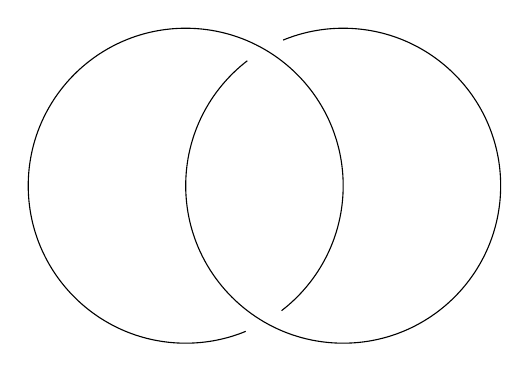
\begin{tikzpicture}
        \path[spath/save=right] (1,0) circle[radius=2cm];
        \path[spath/save=left] (-1,0) circle[radius=2cm];
        \tikzset{
          spath/remove empty components/.list={left,right},
          spath/split at intersections={left}{right},
          spath/insert gaps after components={left}{15pt}{1},
          spath/insert gaps after components={right}{15pt}{2},
          spath/spot weld/.list={left,right},
        }
        \draw[spath/use={left}];
        \draw[black,spath/use={right}];
    \end{tikzpicture}
    }
}
\newcommand{\KP}[1]{%
  \begin{tikzpicture}[baseline=-\dimexpr\fontdimen22\textfont2\relax]
  #1
  \end{tikzpicture}%
}
\newcommand{\KPB}{%
  \KP{
    \draw[color=black,thick] (-0.3,0.3) -- (0.3,-0.3);
    \draw[color=black,thick] (-0.3,-0.3) -- (-0.05,-0.05);
    \draw[color=black,thick] (0.05,0.05) -- (0.3,0.3);
  }%
}
\newcommand{\KPC}{%
  \KP{%
    \draw[color=black,thick] (-0.3,0.3) .. controls (0,-0.05) .. (0.3,0.3);
    \draw[color=black,thick] (-0.3,-0.3) .. controls (0,0.05) .. (0.3,-0.3);
  }%
}
\newcommand{\KPD}{%
  \KP{%
    \draw[color=black,thick] (-0.3,-0.3) .. controls (0.05,0) .. (-0.3,0.3);
    \draw[color=black,thick] (0.3,-0.3) .. controls (-0.05,0) .. (0.3,0.3);
  }%
}
\newcommand{\KPR}{
    \KP{%
    \draw[color=black,thick] (-0.3,-0.3) .. controls (0.05,0) .. (-0.3,0.3);
  }%
}
\newcommand{\KPL}{
    \KP{%
    \draw[color=black,thick] (0.3,-0.3) .. controls (-0.05,0) .. (0.3,0.3);
  }%
}

\usepackage{enumitem}

\tikzset{overcross/.style={double, line width=1.5, white, double=#1, double distance=\knotlinewidth},
    overcross/.default={black},
    knot/.style={line width=\knotlinewidth, baseline=-.5ex}}

\newcommand{\knotlinewidth}{.7pt}
\newcommand{\myarrow}{$\quad\longleftrightarrow\quad$}
\newcommand{\RIa}[1][]{\tikz[knot, #1]{\draw(-.5,.5) to[out=-90,in=-90] (.5,0); \draw[overcross] (.5,0) to[out=90,in=90] (-.5,-.5);}}
\newcommand{\RIb}[1][]{\tikz[knot, #1]{\draw[looseness=.8] (-.5,-.5) to[out=90, in=-90] (.5,0) to[out=90, in=-90] (-.5,.5);}}
\newcommand{\RIIa}[1][]{\tikz[knot, #1]{\draw[red, looseness=2.3] (-.5,-.5) to[out=0, in=0] (-.5,.5); \draw[looseness=2.3, overcross=blue] (.5,-.5) to[out=180, in=180] (.5,.5);}}
\newcommand{\RIIan}[1][]{\tikz[knot, #1]{\draw[black, looseness=2.3] (-.5,-.5) to[out=0, in=0] (-.5,.5); \draw[looseness=2.3, overcross=black] (.5,-.5) to[out=180, in=180] (.5,.5);}}
\newcommand{\RIIb}[1][]{\tikz[knot, #1]{\draw[red, looseness=1.4] (-.5,-.5) to[out=0, in=0] (-.5,.5);\draw[blue, looseness=1.4] (.5,.5) to[out=180,in=180] (.5,-.5);}}
\newcommand{\RIIbn}[1][]{\tikz[knot, #1]{\draw[black, looseness=1.4] (-.5,-.5) to[out=0, in=0] (-.5,.5);\draw[black, looseness=1.4] (.5,.5) to[out=180,in=180] (.5,-.5);}}
\newcommand{\RIIc}[1][]{\tikz[knot, #1]{\draw[blue, looseness=2.3] (.5,-.5) to[out=180, in=180] (.5,.5); \draw[looseness=2.3, overcross=red] (-.5,-.5) to[out=0,in=0] (-.5,.5);}}
\newcommand{\RIIcn}[1][]{\tikz[knot, #1]{\draw[black, looseness=2.3] (.5,-.5) to[out=180, in=180] (.5,.5); \draw[looseness=2.3, overcross=black] (-.5,-.5) to[out=0,in=0] (-.5,.5);}}
\newcommand{\RIIIa}[1][]{\tikz[knot, #1]{\draw[red] (-120:.58) to[out=60,in=-120] (150:.2) to[out=60, in=-120] (60:.58); \draw[rotate=-120, overcross=blue] (-120:.58) to[out=60, in=-120] (150:.2) to[out=60, in=-120] (60:.58); \draw[rotate=120, overcross=green!80!black] (-120:.58) to[out=60, in=-120] (150:.2) to[out=60, in=-120] (60:.58);}}

%%%%%%%%%%%%%%%%%%%%%%%%%%%%%%%%%%%%%%%%%%%%%%%%%%%%%%%%%%%%%%%%%%%%%%%%%%%%%%%%%%%%%%%%%%%%%%%%%%%%%%%%%%%%%%%%%%%%%%%%%%%%%%%%%%%%%%%%%%%%%%%%%%
%%%%%%%%%%%%%%%%%%%%%%%%%%%%%%%%%%%%%%%%%%%%%%%%%%%%%%%%%%%%%%%%%%%%%%%%%%%%%%%%%%%%%%%%%%%%%%%%%%%%%%%%%%%%%%%%%%%%%%%%%%%%%%%%%%%%%%%%%%%%%%%%%%
%%%%%%%%%%%%%%%%%%%%%%%%%%%%%%%%%%%%%%%%%%%%%%%%%%%%%%%%%%%%%%%%%%%%%%%%%%%%%%%%%%%%%%%%%%%%%%%%%%%%%%%%%%%%%%%%%%%%%%%%%%%%%%%%%%%%%%%%%%%%%%%%%%
%%%%%%%%%%%%%%%%%%%%%%%%%%%%%%%%%%%%%%%%%%%%%%%%%%%%%%%%%%%%%%%%%%%%%%%%%%%%%%%%%%%%%%%%%%%%%%%%%%%%%%%%%%%%%%%%%%%%%%%%%%%%%%%%%%%%%%%%%%%%%%%%%%

\title{Exercises}

\begin{document}
\maketitle
\emph{Please note that I do not take credit for all of the Tikz in this document, particularly the knot diagrams. Much of it is taken or templated from online forums such as MathStackExchange}

\section{Categories and Pre-reqs}

\emph{exercise - }\label{PreEx1} Show the forgetful functor \(F: \text{Vect}_k \to \text{Set}\) is a functor.

\emph{proof - } The identity linear transformation is the identity when regarded as a set mapping, if \(T: U \to V, \varphi: V \to S\) as vector spaces, then \(F(\varphi)\circ F(T)\) is a well defined set mapping, which maps \(U \to S\) as sets.

%%%%%%%%%%%%%%%%%%%%%%%%%%%%%%%%%%%%%%%%%%%%%%%%%%%%%%%%%%%%%%%%%%%%%%%%%%%%%%%%%%%%%%%%%%%%%%%%%%%%%%%%%%%%%%%%%%%%%%%%%%%%%%%%%%%%%%%

\emph{exercise - }\label{PreEx2} \(\homo(-,G)\) is functorial

\emph{proof - } Note that if \(f: H \to K\), then \(\homo(-,G)(f) = f^*\) where \(f^*: \homo(K,G) \to \homo(H,G)\) via \(f^*(k) = k \circ f\). We first check associativity, let \(f: H \to K,\; g: K \to N\), and \(z \in \homo(N,G)\), then \((fg)^*(z) = z \circ fg = f^*(z)\circ g = g^*f^*z\).

We can also check that identity is preserved, since if \(f: \homo(H,G) \to \homo(K,G)\) and \(g: \homo(N,G) \to \homo(H,G)\), then for \(h \in \homo(H,G) \tand n \in \homo(N,G)\)
\begin{align*}
    f 1_H^* h = f (n \circ 1_H) = f(h) \tand 1_H^*gn = g(n) \circ 1 = g(n) \qed
\end{align*}

%%%%%%%%%%%%%%%%%%%%%%%%%%%%%%%%%%%%%%%%%%%%%%%%%%%%%%%%%%%%%%%%%%%%%%%%%%%%%%%%%%%%%%%%%%%%%%%%%%%%%%%%%%%%%%%%%%%%%%%%%%%%%%%%%%%%%%%
%%%%%%%%%%%%%%%%%%%%%%%%%%%%%%%%%%%%%%%%%%%%%%%%%%%%%%%%%%%%%%%%%%%%%%%%%%%%%%%%%%%%%%%%%%%%%%%%%%%%%%%%%%%%%%%%%%%%%%%%%%%%%%%%%%%%%%%

\section{Chain Complexes}\label{CCEx} \ref{CCNotes}

\emph{exercise - }\label{CCEx1} Show that \(\mathbf{h} = (h_i)\), \(h_i: C_i \to C_{i+1}'\), then \(h_{i-1}\circ d_i + d_{i+1}' \circ h_i\) is a chain map.

\emph{proof - } We need to check that \(d_i' \circ f_i = f_{i-1} \circ d_i\), in other words we need to show
\begin{align*}
    d_i' \circ (h_{i-1}\circ d_i + d_{i+1}' \circ h_i) = (h_{i-2}\circ d_{i-1} + d_{i}' \circ h_{i-1})\circ d_i
\end{align*}
Since we are in a module, we can distribute \(d_i'\) on the left hand side, rewriting the condition as
\begin{align*}
    d_i' \circ h_{i-1}\circ d_i + d_i' \circ d_{i+1}' \circ h_i = h_{i-2}\circ d_{i-1}\circ d_i + d_{i}' \circ h_{i-1}\circ d_i
\end{align*}
So it will suffice to show that
\begin{align*}
    d_i' \circ d_{i+1}' \circ h_i = h_{i-2}\circ d_{i-1}\circ d_i
\end{align*}
But this is trivial since "\(d^2 = 0\)"


%%%%%%%%%%%%%%%%%%%%%%%%%%%%%%%%%%%%%%%%%%%%%%%%%%%%%%%%%%%%%%%%%%%%%%%%%%%%%%%%%%%%%%%%%%%%%%%%%%%%%%%%%%%%%%%%%%%%%%%%%%%%%%%%%%%%%%%


\emph{exercise - }\label{CCEx2} A homotopy of chains is an equivalence relation

\emph{proof - } We will prove the following items: reflexivity, symmetry, transitivity
\begin{itemize}
    \item To see that \(f \sim f\), take each to be the zero map, \(h_i = 0, \forall i\). In this case the diagram with maps given by \(\mathbf{h}\) is immediate.
    \item Suppose that \(f \sim g\), then we have some \(\mathbf{h}\), such that \(g_i -f_i = h_{i-1}\circ d_i + d_{i+1}' \circ h_i\) for each \(i\). Since \(h_i\) are morphisms of modules, so are \(-h_i\), so in particular we have \(\mathbf{-h} := (-h_i)_i\), so that 
    \begin{align*}
        f_i - g_i &= -(g_i - f_i) = -(h_{i-1}\circ d_i + d_{i+1}' \circ h_i) = -h_{i-1}\circ d_i + -d_{i+1}' \circ h_i \\
        &= -h_{i-1}\circ d_i + d_{i+1}' \circ -h_i
    \end{align*}
    The last line follows since \(d_{i+1}'\) is linear.
    \item Suppose that \(f \sim g \sim r\), and let \(\mathbf{h, k}\) be respective witnesses of these homotopies. Then we have
    \begin{align*}
            &r_i - g_i = k_{i-1}\circ d_i + d_{i+1}'\circ k_i \\
            &g_i - f_i = h_{i-1}\circ d_i + d_{i+1}'\circ h_i
    \end{align*}
    This furnishes
    \begin{align*}
        &r_i - f_i = k_{i-1}\circ d_i + d_{i+1}'\circ k_i + h_{i-1}\circ d_i + d_{i+1}'\circ h_i
                   = (k_{i-1} + h_{i-1})\circ d_i + d_{i+1}'\circ(h_i + k_i)
    \end{align*}
    So we have the homotopy \(r \sim f\) via \(\mathbf{h} + \mathbf{k}\), we are done since we already proved symmetry.
\end{itemize}


%%%%%%%%%%%%%%%%%%%%%%%%%%%%%%%%%%%%%%%%%%%%%%%%%%%%%%%%%%%%%%%%%%%%%%%%%%%%%%%%%%%%%%%%%%%%%%%%%%%%%%%%%%%%%%%%%%%%%%%%%%%%%%%%%%%%%%%


\emph{exercise - }\label{CCEx3} Show that the following two chain complexes are homotopic:
\begin{equation*}
    \begin{tikzcd}
        0 \arrow[r] & \mathbf{Z} \oplus \mathbf{Z} \arrow[r,"{(\cdot , 2\cdot)}"] & \mathbf{Z} \oplus \mathbf{Z} \arrow[r] & 0 \oplus \mathbf{Z}/(2) \arrow[r] & 0 \\
        0 \arrow[r] & \mathbf{Z} \arrow[r,"2\cdot"] & \mathbf{Z} \arrow[r] & \mathbf{Z}/(2) \arrow[r] & 0
    \end{tikzcd}
\end{equation*}

\emph{proof - } Let each \(f_i\) be the projection of the second coordinate, and each \(g_i\) the inclusion into the second coordinate. In thise case we have
\begin{align*}
    \mathbf{1}_{C'} - \mathbf{fg} = \mathbf{0}
\end{align*}
and hence \(\mathbf{h} = (0)_i\) witnesses the homotopy. The slightly harder case is the other direction. Define \(h_2 = h_0 = h_{-1} = 0\), and \(h_1: (m,n) \mapsto m\). By definition of \(\mathbf{f}, \mathbf{g}\), we have \(1_{C,i} - g_if_i: (m,n) \mapsto (m,0)\), so we just need to check that our given \(\mathbf{h}\) satisfies this.
\begin{align*}
    &(d_3h_2 + h_1d_2)(m,n) = 0 + h_1(m,2n) = (m,0) \\
    &(d_2h_1 + h_0d_1)(m,n) = d_2(m,0) + 0 = (m,0) \\
    &(d_1h_0 + h_{-1}d_0)(0,n) = 0 + 0 = (0,0)
\end{align*}
This verifies the homotopy.


%%%%%%%%%%%%%%%%%%%%%%%%%%%%%%%%%%%%%%%%%%%%%%%%%%%%%%%%%%%%%%%%%%%%%%%%%%%%%%%%%%%%%%%%%%%%%%%%%%%%%%%%%%%%%%%%%%%%%%%%%%%%%%%%%%%%%%%


\textbf{Theorem - }\label{CCEx4} ("\emph{The Fundamental Theorem of Homology For Chain Complexes}") If chain complexes \(C,C'\) are homotopic, then they have the same Homology Modules.

\emph{proof - } Recall that
\begin{align*}
    H^i := \frac{\ker(d_i)}{\im(d_{i+1})}
\end{align*}
Now let the homotopy be given by \(\mathbf{f}:C \to C', \mathbf{g}:C' \to C\), there is a natural induced map of \(f_i\) on \(H^i\), given by restricting \(f_i\) to \(\im(d_{i+1})\), then taking the unique map from the quotient by the kernel of \(d_i\), which exists and is unique by the first isomorphism theorem. Calling this induced map \(f_{i,*}\), we need to check that
\(f_{i,*}\) maps into \(H_i'\). First it is immediate that \(f_i\vert_{\ker{d_i}}: \ker d_i \to \ker d_i'\), since \(d_i'f_i = f_{i-1}d_i\), where the right hand side is zero when restricted to \(\ker(d_i)\), well definition on cosets follows from "\(d^2 = 0\)". So only need check that \((hd + dh)_* = 0\), \(d_{i+1}h \in \text{Im}\, d_{i+1} = 0\) so it only remains to show that \(hd_i = 0\) on \(\ker d_i\), this is trivial since \(h(0) = 0\) and for any \(z \in \ker d_i\) \(hd_i(z) = h(0)\). \qed


%%%%%%%%%%%%%%%%%%%%%%%%%%%%%%%%%%%%%%%%%%%%%%%%%%%%%%%%%%%%%%%%%%%%%%%%%%%%%%%%%%%%%%%%%%%%%%%%%%%%%%%%%%%%%%%%%%%%%%%%%%%%%%%%%%%%%%%
%%%%%%%%%%%%%%%%%%%%%%%%%%%%%%%%%%%%%%%%%%%%%%%%%%%%%%%%%%%%%%%%%%%%%%%%%%%%%%%%%%%%%%%%%%%%%%%%%%%%%%%%%%%%%%%%%%%%%%%%%%%%%%%%%%%%%%%


\section{Homology and Cell Complexes}

\emph{exercise - }\label{HEx1} Let \(G\) be a graph, then \(\ker d_1 = \set{\text{Cycles in }G}\)

\emph{proof - } We have the map \(d_1: \oplus_i \mathbf{Z}e_i \to \oplus_i \mathbf{Zv_i}\), then \(\sum_i k_i e_i \in \ker d_1 \iff \sum_i k_i (H(e_i) - T(e_i)) = 0\), where \(H(e)\) denotes the target of an edge, and \(T(e)\) denotes the source of an edge. Then \(\sum_i k_i (H(e_i) - T(e_i)) = \sum_j\ell_j v_j = 0 \iff \ell_j = 0,\; \forall j\). Where \(\ell_j = \sum_{\set{e_i \mid v_j = H(e_i)}} k_i - \sum_{\set{e_i \mid v_j = T(e_i)}} k_i\) so that \(\ell_j = 0\) for all \(j\) exactly when every vertex has an equal number of in and out edges. \qed

%%%%%%%%%%%%%%%%%%%%%%%%%%%%%%%%%%%%%%%%%%%%%%%%%%%%%%%%%%%%%%%%%%%%%%%%%%%%%%%%%%%%%%%%%%%%%%%%%%%%%%%%%%%%%%%%%%%%%%%%%%%%%%%%%%%%%%%

\emph{exercise - }\label{HEx2} Show that for the graph \(G\), with \(V(G) = \set{x,y}, E(G) = \set{a = (x,y),b = (x,y), c = (x,y)}\) we have \(\ker d_1 = \gen{a-b, b-c}\)

\emph{proof - } Here we have \(d_1: a,b,c \mapsto y-x\), then \(a-b, b-c \in \ker d_1\). We have \(d_1: n_1a + n_2b + n_3c \mapsto (n_1 + n_2 + n_3)(x-y)\), so that \(\ker d_1 = \set{na + mb + k\ell \mid n + m + \ell = 0}\), so fixing \(na + mb + k\ell = na + mb + -(n+m)c \in \ker d_1\), we have \(na + mb + k\ell = n(a-b) + (m+n)(b-c) \in (a-b,b-c)\) \qed

%%%%%%%%%%%%%%%%%%%%%%%%%%%%%%%%%%%%%%%%%%%%%%%%%%%%%%%%%%%%%%%%%%%%%%%%%%%%%%%%%%%%%%%%%%%%%%%%%%%%%%%%%%%%%%%%%%%%%%%%%%%%%%%%%%%%%%%

\emph{exercise - }\label{HEx3} Consider the following Graph:

\begin{equation}
        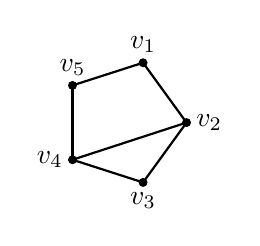
\begin{tikzpicture}[scale=0.8]
                \coordinate (b) at (0.31,0.95);
                \coordinate (c) at (1,0);
                \coordinate (d) at (0.31,-0.95);
                \coordinate (e) at (-0.81,-0.59);
                \coordinate (f) at (-0.81,0.59);
    
                \draw[fill] (b) circle (1.75pt);
                \draw[fill] (c) circle (1.75pt);
                \draw[fill] (d) circle (1.75pt);
                \draw[fill] (e) circle (1.75pt);
                \draw[fill] (f) circle (1.75pt);
    
                \draw[thick] (b)--(c);
                \draw[thick] (c)--(d);
                \draw[thick] (d)--(e);
                \draw[thick] (e)--(f);
                \draw[thick] (b)--(f);
                \draw[thick] (c)--(e);
                
                \node[above] at (0.31,0.95) {\(v_1\)};
                \node[right] at (1,0) {\(v_2\)};
                \node[below] at (0.31,-0.95) {\(v_3\)};
                \node[left] at (-0.81,-0.59) {\(v_4\)};
                \node[above] at (-0.81,0.59) {\(v_5\)};
    \end{tikzpicture}
    \end{equation}

    Where the edges are oriented with the larger vertex index at the head and smaller at the tail. Compute generators for the cycles, and show that \(C_*(G) \simeq C_*(G')\) as chain complexes, where \(G'\) is \(G\) with \((v_1,v_5)\) replaced with \((v_5,v_1)\). Finally, show that \(H_1(G) \cong H_1(G')\)
    
    \emph{proof - }
    We can write \(d_1\) as a matrix,
    \begin{align*}
        \begin{bmatrix} -1 & 0 &0 &0 &0 &-1 \\ 1 &-1 &-1 &0 &0 &0  \\ 0 & 1& 0&-1&0 &0  \\ 0 &0 &1 &1 &-1 &0 \\ 0 & 0&0 &0 & 1& 1 \end{bmatrix} \overset{\text{Row Reduction}}{\rightsquigarrow} \begin{bmatrix} -1&0&0&0&0&-1\\0&-1&-1&0&0&-1\\0&0&-1&-1&0&-1\\0&0&0&0&-1&-1\\0&0&0&0&0&0\end{bmatrix}
    \end{align*}
    So the kernel has rank 2.
    From this matrix we can compute generators for the kernel, (and thus the cycles)
    \[\ker d_1 = (e_2-e_4,e_1+e_5-e_6)\]

    To show that \(C_*(G)\), and \(C_*(G')\) are chain homotopic, define \[f:v_i \mapsto v_i', e_i \mapsto e_i', \quad g: v_i' \mapsto v_i, e_i' \mapsto e_i\].
    By construction these are chain maps, since firstly \(d_0 = 0, d_0' = 0\), and \(e_i = e_i'\) for each \(e_i \neq (v_1,v_5)\), and the values of \(d_1\) agree with \(d_1'\) on each of the equal \(e_i = e_i'\). For \(e = (v_1,v_5), e' = (v_5,v_1)\), we have \(f_1(e) = -e',g_1(e')=-e\), for \(e \neq (v_1,v_5), e' \neq (v_5,v_1)\) commutativity is obvious since \(d(e) = d'(e')\) in this case. For \(e = (v_1,v_5)\) we have \(f_0 \circ d(e) = f_0(x-y) = x-y = -(y-x) = -d_1'(e') = d_1'(f_1(e))\), the argument is the exact same for commutativity of the square replacing \(g\) for \(f\) and \(e'\) for \(e\). Then \(f \circ g = 1\), so we can just choose our homotopy to be the zero map.

    To see that the homology is the same, there are 2 possible solutions both are easy. The first is that they are isomorphic as chain complexes, the second is that \(d_1\) is rewritten by multiplying a row by \(-1\), preserving the row reduced form and hence the generators of the kernel. \qed



    %%%%%%%%%%%%%%%%%%%%%%%%%%%%%%%%%%%%%%%%%%%%%%%%%%%%%%%%%%%%%%%%%%%%%%%%%%%%%%%%%%%%%%%%%%%%%%%%%%%%%%%%%%%%%%%%%%%%%%%%%%%%%%%%%%%%%%%

    
    \emph{exercise - }\label{HEx4} Let \(\Gamma, \Gamma'\) be arbitrary graphs such that \(\Gamma \simeq \Gamma'\), then \(C_*(\Gamma) \simeq C_*(\Gamma')\)

    \emph{proof - } In (i) we show that homotopy of graphs is independent of orientation, and in (ii), we show that it is equivalent up to quotienting by an edge between to vertices, this is sufficient since it allows us to show that (since the graphs are homotopic they have the same Euler characteristic)
    \[C_*(\Gamma) \simeq C_*(\bigvee_{1 \leq k \leq \chi(\Gamma)} S^1) \simeq C_*(\Gamma')\]

    (i) Assume that \(\Gamma\setminus e_0 = \Gamma' \setminus e_0'\), such that \(e_0' = -e_0\), we copy the proof in the previous question.
    \begin{align*}
        f: &C_*(\Gamma) \to C_*(\Gamma')
        &\begin{cases}
            e_0 \mapsto -e_0' \\
            e_i \mapsto e_i' & i \geq 1 \\
            v_i \mapsto v_i'
        \end{cases}
        g: &C_*(\Gamma') \to C_*(\Gamma)
        &\begin{cases}
            e_0' \mapsto -e_0 \\
            e_i' \mapsto e_i & i \geq 1 \\
            v_i' \mapsto v_i
        \end{cases}
    \end{align*}
    \(fg = 1_{C_*(\Gamma)}\), \(gf = 1_{C_*(\Gamma')}\), so they are homotopies so long as they are chain maps. This is trivial except for the "square" where edges map to vertices.
    Commutativity on generators is trivial apart from \(e_0\), and \(e_0'\), in this case \(f\circ d_1(e_0) = f(v_1 - v_0) = v_1' - v_0' = -(v_0' - v_1') = d_1'(-e_0') = d_1'\circ f (e_0)\). The proof is the same for \(g\).

    (ii) Suppose we are quotienting the edge \(e_0 = (v_0,v_1), v_0 \neq v_1\). Here in order to focus on the most relevant parts of the chain complex we do some book keeping:
    \begin{align*}
        &C_*(\Gamma)_2 = \mathbb{Z}_0^2 \oplus S_2 &C_*(\Gamma)_1 = \mathbb{Z}_0^1 \oplus \mathbb{Z}_1^1 \oplus S_1 \\
        &C_*(\Gamma')_2 = S_2' &C_*(\Gamma')_1 = \mathbb{Z}_0' \oplus S_1'
    \end{align*}
    Here there are natural identifications of all edges and vertices in \(S_i \tand S_i'\). There is really only one way to define \(f\) if we want to keep the natural mapping \(f: S_i \to S_i'\),
    \begin{align*}
        &f_1: (a_0e_0,a_1e_1,\hdots,a_me_m) \mapsto (a_1\overline{e_1},a_2\overline{e_2},\hdots,a_m\overline{e_m}) \\
        &f_0:(a_0v_0,a_1v_1,\hdots,a_nv_n) \mapsto ((a_0+a_1)\overline{v_1},a_2\overline{v_2},\hdots,a_n\overline{v_n})
    \end{align*}
    It is clear that \(f\) is a chain map from construction. Now we define \(g: C_*(\Gamma') \to C_*(\Gamma)\) as follows,
    \begin{align*}
        g_0: (a_1\overline{v_1},\hdots,a_n\overline{v_n}) \mapsto (0,a_1v_1,\hdots,a_nv_n)
    \end{align*}
    Then taking the natural map \(S_2' \to S_2\), composition with \(d\) gives \(e_i \mapsto \sum_{j=0}^nk_j^iv_j\), define \(g_1: \overline{e_i} \mapsto k^i_0e_0 + e_i\). Then we have \(\overline{k_1^i} = k_0^i + k_1^i\)
    \[d_1g_1(\overline{e_i}) = d_1(k_0^ie_0 + e_i) = k_0^i(v_1 - v_0) + \sum_{j=0}^n k_j^i v_j\]
    \[g_0\overline{d_1}(\overline{e_i}) = g_0\left(\sum_{j=1}^n \overline{k_j^i} \overline{v_j}\right) = g_0\left((k_0^i + k_1^i)\overline{v_1} + \sum_{j=2}^n k_j^i \overline{v_j}\right) = \sum_{j=0}^n k_j^i v_j + k_0^i(v_1 - v_0)\]
    This implies that \(g\) is indeed a chain map. It is immediate that \(fg = 1_{C_*(\Gamma')}\), we need to provide a homotopy to show that \(gf \simeq 1_{C_*(\Gamma)}\). Explicitly we have
    \begin{align*}
        &1 - g_1f_1 = \left(a_0 - \sum_1^m a_i k_0^i\right)e_0 \\
        &1 - g_0f_0 = a_0(v_0 - v_1)
    \end{align*}
    the map \(h: v_0 \mapsto -e_0\) obviously satisfies \(d_1h_1(a_0,\hdots,a_n) = a_0(v_0 - v_1)\). We only need to check that \(h_1d_1 = \left(a_0 - \sum_1^m a_i k_0^i\right)e_0\), but the first coordinate of \(d_1(a_0e_0 + \sum_{i=1}^m a_i e_i)\) is \(-a_0 + \sum_{i=1}^m a_ik_0^i\), by definition of \(k_0^i\), and since \(e_0 = (v_0,v_1)\). It follows that \[h_1\circ d_1(a_0e_0 + \sum_{i=1}^m a_i e_i) = -(-a_0 + \sum_{i=1}^m a_ik_0^i)e_0 = 1-g_1f_1 \qed\]

    %%%%%%%%%%%%%%%%%%%%%%%%%%%%%%%%%%%%%%%%%%%%%%%%%%%%%%%%%%%%%%%%%%%%%%%%%%%%%%%%%%%%%%%%%%%%%%%%%%%%%%%%%%%%%%%%%%%%%%%%%%%%%%%%%%%%%%%


    \emph{exercise - }\label{HEx5} Using the cell structures for \(S^2\) from \(e^2 \cup e^0\), \(e^2 \cup e^2 \cup e^1 \cup e^0\) Build \(C_*(S^2)\) and compute its Homology.

    \emph{proof - } The first cell structure gives the sequence

    \begin{equation*}
        \begin{tikzcd}
            0 \arrow[r] & \mathbb{Z} \arrow[r] & 0 \arrow[r] & \mathbb{Z} \arrow[r] & 0
        \end{tikzcd}
    \end{equation*}

    In this case the homology modules are trivially \(H_i(C_*(S^2)) = \begin{cases}
        0 & i \neq 0,2 \\
        1 & i = 0,2
    \end{cases}\)

    The second cell structure gives the sequence

    \begin{equation*}
        \begin{tikzcd}
            0 \arrow[r] & \mathbb{Z}e_0^2 \oplus \mathbb{Z}e_1^2 \arrow[r,"{d_2}"] & \mathbb{Z}e_0^1 \arrow[r,"{d_1}"] & \mathbb{Z}e_0^0 \arrow[r] & 0
        \end{tikzcd}
    \end{equation*}

    Where \(\mathbb{Z}e_0^2 \oplus \mathbb{Z}e_1^2 = \mathbb{Z}\gen{e_0^2 + e_1^2} \oplus \mathbb{Z}\gen{e_0^2 - e_1^2}\), and \(d_2: e_0^2 \mapsto e_0^1, e_1^2 \mapsto -e_0^1\), so that
    \begin{align*}
        H_2(C_*(S^2)) = \frac{\mathbb{Z}\gen{e_0^2 + e_1^2} \oplus \mathbb{Z}\gen{e_0^2 - e_1^2}}{\mathbb{Z}\gen{e_0^2 + e_1^2}} \cong \mathbb{Z}
    \end{align*}
    And \(d_1: e_0^1 \mapsto e_0^0 - e_0^0\), so that \(d_1 \equiv 0\) which gives us \(H_0(C_*(S^2)) = \mathbb{Z}\), and \(H_1(C_*(S^2)) = \mathbb{Z}/\mathbb{Z} \cong 0\), with \(H_i = 0\) for \(i > 2\). The same result as above.
    



    %%%%%%%%%%%%%%%%%%%%%%%%%%%%%%%%%%%%%%%%%%%%%%%%%%%%%%%%%%%%%%%%%%%%%%%%%%%%%%%%%%%%%%%%%%%%%%%%%%%%%%%%%%%%%%%%%%%%%%%%%%%%%%%%%%%%%%%

    \emph{exercise - }\label{HEx6} Show that "augmentation" still gives a chain complex, i.e. \(\epsilon\circ d_1 = 0\)

    \emph{proof - } It will suffice to check on generators of \(C_1\), let \(e^1_\beta \in C_1\), then 
    \[\epsilon d_1(e^1_\beta) = \epsilon (e_\alpha^0 - e_{\beta}^0) = \epsilon(e_\alpha^0) - \epsilon(e_\beta^0) = 1-1 = 0\]

    %%%%%%%%%%%%%%%%%%%%%%%%%%%%%%%%%%%%%%%%%%%%%%%%%%%%%%%%%%%%%%%%%%%%%%%%%%%%%%%%%%%%%%%%%%%%%%%%%%%%%%%%%%%%%%%%%%%%%%%%%%%%%%%%%%%%%%%

    \emph{exercise - }\label{HEx7} \(S^1 \wedge S^1 \simeq S^2\)

    \emph{proof - } \(S^1 \wedge S^1 \cong \frac{T^2}{S^1 \vee S^1}\), where \(T^2 \cong D^2/\sim\), then
    \begin{align*}
        S^1 \wedge S^1 = \frac{T^2}{S^1 \vee S^1} \cong \frac{D^2/\sim}{\partial D^2} = \frac{D^2}{\partial D^2} \cong S^2
    \end{align*}

    %%%%%%%%%%%%%%%%%%%%%%%%%%%%%%%%%%%%%%%%%%%%%%%%%%%%%%%%%%%%%%%%%%%%%%%%%%%%%%%%%%%%%%%%%%%%%%%%%%%%%%%%%%%%%%%%%%%%%%%%%%%%%%%%%%%%%%%

    \emph{exercise - }\label{HEx8} \(SX \simeq \sum X\)

    \emph{proof - } Here \((X,\set{*})\) is a (pointed but ignore the point for now) CW-complex, we can give \(X \times I\) a CW structure, note that we have \(\partial e^n = \partial(e^{n-1} \times I) = (\partial e^{n-1} \times I)\cup e^{n-1} \times \partial I\)
    (we can do this using point set topology and the fact that the sets are closed), then the CW-structure on \((X \times I)^n\) can be taken to be \((X \times I)^0 = X^0 \times \partial I\), then taking \(\varphi_\alpha^n\) to be the gluing map of \(e_\alpha^{n}\) into \(X^n\):
    \begin{align*}
        (X \times I)^n = (X \times I)^{n-1} \bigcup_{\varphi_\alpha^n} e_\alpha^n \times \partial I \bigcup_{\varphi_\alpha^{n-1} \times I} e_\alpha^{n-1} \times I
    \end{align*}
    This gives a CW structure on \(X \times I\) with \(X \times \partial I\) as a substructure, there is a canonical CW structure on the quotient given by replacing \(\varphi_\alpha^n\) with \(\pi\vert_{X^n} \circ\varphi_\alpha^n\). Furthermore since \(* \in X^0\), we have \(\set{*} \times I \in (X \times I)^1\), which can be identified with its image in the quotient. This is a contractible subcomplex, so by the CW extension theorem
    \begin{align*}
        SX = \frac{X \times I}{X \times \partial I} \cong \frac{X \times I}{X \times \partial I \cup \set{*} \times I} = \sum X
    \end{align*}
    
    %%%%%%%%%%%%%%%%%%%%%%%%%%%%%%%%%%%%%%%%%%%%%%%%%%%%%%%%%%%%%%%%%%%%%%%%%%%%%%%%%%%%%%%%%%%%%%%%%%%%%%%%%%%%%%%%%%%%%%%%%%%%%%%%%%%%%%%

    \emph{exercise - }\label{HEx9} \(X \wedge S^1 \simeq \sum X\)

    \emph{proof - } It is important here that the same point \(x \in X\) is used in either quotient. Consider the map \(f: I \to S^1, t \mapsto e^{i\pi t}\), then we get the following,
    \begin{equation*}
        \begin{tikzcd}
            X \times I \arrow[d,"{\pi}"] \arrow[r,"{1 \times f}"] & X \times S^1 \arrow[d,"{\pi'}"] \\
            \frac{X \times I}{X \times \set{1} \cup X \times \set{-1} \cup \set{x}\times I} \arrow[r,"{\overline{1 \times f}}"] &\frac{X \times S^1}{X\times \set{1} \cup \set{x} \times S^1}
        \end{tikzcd}
    \end{equation*}

    The bottom left here is the (reduced) suspension \(\sum X\), and the bottom right is \(X \wedge S^1\). Here the induced map is clearly bijective, since the quotients here are equivalent to quotienting by the image of the quotients, along with quotienting on the left side \(f^{-1}(1) \times \set{1} \sim f^{-1}(-1) \times \set{-1} \sim x\), where \(f\) wasn't injective. Continuity of the inverse follows, since we have \(\frac{X \times I}{X \times \partial I} \cong \frac{X \times S^1}{X \times 1}\), and we can factor our map through this homeomorphism before taking quotients.
    %%%%%%%%%%%%%%%%%%%%%%%%%%%%%%%%%%%%%%%%%%%%%%%%%%%%%%%%%%%%%%%%%%%%%%%%%%%%%%%%%%%%%%%%%%%%%%%%%%%%%%%%%%%%%%%%%%%%%%%%%%%%%%%%%%%%%%%

    \emph{exercise - }\label{HEx10} Use \(\tilde{H_i}\) to show that \(\partial D^n\) cannot be a retract of \(D^n\)

    \emph{proof - } We have that \(D^n/\partial D^n \cong S^n\), furthermore \(D^n \simeq \set{x}\) for all \(n\), implying that \(\tilde{H}_i(D^n) \cong \tilde{H}_i(\set{x}) = 0\), for any \(i,n \in \mathbb{Z}_{\geq 0}\). Suppose for contradiction that there were a retract \(h: D^n \to \partial D^n\), then denoting \(\iota: \partial D^n \hookrightarrow D^n\) we would have that \(h \circ \iota \simeq 1_{\partial D^n}\), by functoriality we get the following commutative diagram (also note that \(\partial D^n = S^{n-1}\)):

    \begin{equation*}
        \begin{tikzcd}
            \tilde{H}_{n-1}(\partial D^n) \arrow[r,"{1}"] \arrow[d,"{\iota_*}"] &\tilde{H}_{n-1}(\partial D^n) \\
            \tilde{H}_{n-1}(D^n) \arrow[ur,"{h_*}"]
        \end{tikzcd}
    \end{equation*}
    Where this diagram is equivalent to
    \begin{equation*}
        \begin{tikzcd}
            \mathbb{Z} \arrow[r,"{1}"] \arrow[d] &\mathbb{Z} \\
            0 \arrow[ur]
        \end{tikzcd}
    \end{equation*}
    This is clearly a contradiction since there are no surjective morphisms \(0 \to \mathbb{Z}\). \qed

    % \begin{equation*}
    %     \begin{tikzcd}
    %         \tilde{H}_n(\partial D^n) \arrow[r] & \tilde{H}_n(D^n) \arrow[r] & \tilde{H}_n(D^n/\partial D^n) \arrow[r] & \tilde{H}_{n-1}(\partial D^n) \arrow[r] & \tilde{H}_{n-1}(D^n) \arrow[r] & \tilde{H}_{n-1}(D^n/\partial D^n) \\
    %         \tilde{H_n}(S^{n-1}) \arrow[r] & \tilde{H_n}(D^n) \arrow[r] & \tilde{H_n}(S^n) \arrow[r] & \tilde{H}_{n-1}(S^{n-1}) \arrow[r] &\tilde{H}_{n-1}(D^n) \arrow[r] & \tilde{H}_{n-1}(S^n)\\
    %         0 \arrow[r] & \tilde{H_n}(D^n) \arrow[r] & \mathbb{Z} \arrow[r] & \mathbb{Z} \arrow[r] &\tilde{H_{n-1}}(D^n) \arrow[r] & 0
    %     \end{tikzcd}
    % \end{equation*}

    %%%%%%%%%%%%%%%%%%%%%%%%%%%%%%%%%%%%%%%%%%%%%%%%%%%%%%%%%%%%%%%%%%%%%%%%%%%%%%%%%%%%%%%%%%%%%%%%%%%%%%%%%%%%%%%%%%%%%%%%%%%%%%%%%%%%%%%

    \emph{exercise - }\label{HEx11} Let \(f: S^n \to S^n\), show if \(f\) is not surjective then \(\deg f = 0\)

    \emph{proof - } Suppose that \(f\) is not surjective, then we can pick some \(x \in S^n \setminus f(S^n)\), by the stereographic projection \(S^n \setminus \set{x} \cong \mathbb{R}^n \simeq \set{*}\), so we have the following commutative diagram, where the downward map is taken by restricting the codomain of \(f\) to \(S^n \setminus \set{x}\), and the upper diagonal is the inclusion.
    \begin{equation*}
        \begin{tikzcd}
            \tilde{H_n}(S^n) \arrow[r,"{f_*}"] \arrow[d] &\tilde{H_n}(S^n) \\
            \tilde{H_n}(\set{*}) \arrow[ur]
        \end{tikzcd}
    \end{equation*}
    equivalently,
    \begin{equation*}
        \begin{tikzcd}
            \mathbb{Z} \arrow[r,"{f_*}"] \arrow[d] &\mathbb{Z} \\
            0 \arrow[ur]
        \end{tikzcd}
    \end{equation*}
    so \(f_*\) must be the zero map.

    %%%%%%%%%%%%%%%%%%%%%%%%%%%%%%%%%%%%%%%%%%%%%%%%%%%%%%%%%%%%%%%%%%%%%%%%%%%%%%%%%%%%%%%%%%%%%%%%%%%%%%%%%%%%%%%%%%%%%%%%%%%%%%%%%%%%%%%

    \emph{exercise - }\label{HEx12} Let \(f\) as in the previous exercise, show that \(\deg f = \deg \sum_* f \) (remark first  show that the suspension \(\sum\) is functorial)

    \emph{proof - } given \(f: X \to Y\), we can define \(\sum_* f\) as the induced map in the following diagram
    \begin{equation*}
        \begin{tikzcd}
            X \times I \arrow[d,"{\pi_X}"] \arrow[r,"{f \times 1}"]& Y \times I \arrow[d,"\pi_Y"] \\
            \sum X \arrow[r,"{\sum_* f}"]& \sum Y
        \end{tikzcd}
    \end{equation*}
    Continuity simply follows from continuity of \(f\), and the definition of quotient topology taking opens to opens on the upper half of the square, then commutativity and the universal property of the quotient on the lower square. To get \(\sum_* fg = \sum_*f \sum_*g\) simply factor \(f\circ g \times 1\) through the following diagram
    \begin{equation*}
        \begin{tikzcd}
            X \times I \arrow[d,"{\pi_X}"] \arrow[r,"{f \times 1}"]& Y \times I \arrow[d,"\pi_Y"] \arrow[r,"{g \times 1}"] &Z \times I \arrow[d,"{\pi_Z}"] \\
            \sum X \arrow[r,"{\sum_* f}"]& \sum Y \arrow[r,"{\sum_* g}"]& \sum Z
        \end{tikzcd}
    \end{equation*}
    \(\sum_*1 = 1_{\sum_*}\) is obvious. This suffices to show functoriality.

    For the proof of the main result, note that by an identical construction, the canonical \(C_*\) is functorial, \(f: X \to Y\), then \(C_*f : C_{1_X} \to C_{1_Y}\). It suffices to show the following result for \(SX\), since it has the same Homology as \(\sum X\) by homotopy equivalence, so factoring \(f\) through this equivalence won't affect the degree. We have naturality (identifying \(S^n \leftrightarrow S^n \times \set{0} f \leftrightarrow C_*f \vert_{S^n \times \set{0}}\))
    \begin{equation*}
        \begin{tikzcd}
            S^n \arrow[d,"{f}"] \arrow[r]& CS^n\arrow[d,"{C_*f}"]\\
            S^n \arrow[r]& CS^n 
        \end{tikzcd}
    \end{equation*}
    And hence, we get a chain map
    \begin{equation*}
        \begin{tikzcd}
            H_{n+1}(CS^n) \arrow[d,"{(C_*f)_*}"] \arrow[r,"{}"]& H_{n+1}(CS^n,S^n) \arrow[d,"{(S_*f)_*}"]\arrow[r,"{}"]& H_n(S^n)\arrow[d,"{f_*}"] \arrow[r,"{}"]& H_n(CS^n) \arrow[d,"{(C_*f)_*}"] \\
            H_{n+1}(CS^n)\arrow[r,"{}"]& H_{n+1}(CS^n,S^n) \arrow[r,"{}"]& H_n(S^n) \arrow[r,"{}"]& H_n(CS^n)
        \end{tikzcd}
    \end{equation*}
    Which we can rewrite as
    \begin{equation*}
        \begin{tikzcd}
            0 \arrow[d,"{(C_*f)_*}"] \arrow[r,"{}"]& H_{n+1}(S(S^n)) \arrow[d,"{(S_*f)_*}"]\arrow[r,"{}"]& H_n(S^n)\arrow[d,"{f_*}"] \arrow[r,"{}"]& 0 \arrow[d,"{(C_*f)_*}"] \\
            0\arrow[r,"{}"]& H_{n+1}(S(S^n)) \arrow[r,"{}"]& H_n(S^n) \arrow[r,"{}"]& 0
        \end{tikzcd}
    \end{equation*}
    Commutativity suffices to show that the degrees of the maps must be equal. \qed
    
    \textbf{Remark 1.} Use of the \(0\) maps on either end of the sequence is a bit of a cheat here so we get for free that \(H_{n+1}(S(S^n)) \cong \mathbb{Z}\), and we need to ensure the map \(H_{n+1}(S(S^n)) \to H_n(S^n)\) is nonzero since otherwise we cannot conclude about \((\sum_*f)_*(1) = (S_*f)_*(1)\) from the above diagram.

    \textbf{Remark 2.} To make sense of degree here we should really show that \(\sum S^n \simeq S(S^n) \simeq S^{n+1}\), there is an explicit homeomorphism by simply rescaling by the factor in \(I\) in \(S^n \times I\), then taking the quotient.


    %%%%%%%%%%%%%%%%%%%%%%%%%%%%%%%%%%%%%%%%%%%%%%%%%%%%%%%%%%%%%%%%%%%%%%%%%%%%%%%%%%%%%%%%%%%%%%%%%%%%%%%%%%%%%%%%%%%%%%%%%%%%%%%%%%%%%%%

    \emph{exercise - }\label{HEx13} Compute the Homology of \(X\), where \(X\) is the triangulation of the Torus.

    \emph{proof - } Let the upper triangle be \(e_U^2\), the lower triangle be \(e_L^2\), the upper/lower boundary be \(e_\alpha^1\), the left/right boundary be \(e_\beta^1\), and the diagonal be \(e_\gamma^1\), there is only one zero-cell, we may call it \(e^0\). Then:
    \begin{align*}
        \pi_\alpha \varphi_U = \pi_\beta \varphi_U = 1 = - \pi_\gamma \varphi_U \\
        \pi_\alpha \varphi_L = \pi_\beta \varphi_L = -1 = - \pi_\gamma \varphi_L \\
        \pi_0 \varphi_\alpha = \pi_0 \varphi_\beta = \pi_0 \varphi_\gamma = 1 - 1 = 0
    \end{align*}

    In this case we have the cell structure
    \begin{equation*}
        \begin{tikzcd}
            0 \arrow[r] & \mathbb{Z}\gen{e^2_U} \oplus \mathbb{Z}\gen{e^2_L} \arrow[r,"{d_2}"] & \mathbb{Z} \gen{e^1_\alpha} \oplus \mathbb{Z} \gen{e^1_\beta} \oplus \mathbb{Z} \gen{e^1_\gamma} \arrow[r,"{d_1}"] &\mathbb{Z} \gen{e^0} \arrow[r] & 0
        \end{tikzcd}
    \end{equation*}
    Where \(\ker d_2 = e_U^2 + e_L^2\), \(d_1 = 0 = d_0\), rewriting \(C_1(X)\) to have \(\text{Im}\,C_2(X)\) as one of its three generators, we get the usual Homology modules for the Torus
    \begin{align*}
        H_2(X) \cong \mathbb{Z}, \quad H_1(X) \cong \mathbb{Z} \oplus \mathbb{Z}, \quad H_0(X) \cong \mathbb{Z}
    \end{align*}


    %%%%%%%%%%%%%%%%%%%%%%%%%%%%%%%%%%%%%%%%%%%%%%%%%%%%%%%%%%%%%%%%%%%%%%%%%%%%%%%%%%%%%%%%%%%%%%%%%%%%%%%%%%%%%%%%%%%%%%%%%%%%%%%%%%%%%%%

    \emph{exercise - }\label{HEx14} Show from the Homology axioms that \(\tilde{H_n}(X^{n+1}) = \tilde{H_n}(X)\)

    \emph{proof - } We have from Axiom 1, the following sequence is exact
    \begin{equation*}
        \begin{tikzcd}
            \tilde{H}_{k+1}(X^{m+1}/X^m) \arrow[r] & \tilde{H}_{k}(X^m) \arrow[r] & \tilde{H}_{k}(X^{m+1}) \arrow[r] & \tilde{H}_{k}(X^{m+1}/X^m)
        \end{tikzcd}
    \end{equation*}
    We have the following from construction of a CW complex:
    \begin{align*}
        X^{n+1}/X^n = \frac{\frac{e_\alpha^{n+1} \bigsqcup_\alpha X^n}{x \sim \varphi_\alpha(x),\; x \in \partial e_\alpha^{n+1},\; \varphi_\alpha(x) \in X^n}}{X^n} = \frac{\bigsqcup_\alpha e_\alpha^{n+1}}{\bigsqcup_{\alpha}\partial e_\alpha^{n+1}} \cong \bigvee_\alpha S^{n+1}
    \end{align*}
    So for \(k \neq m+1,m\) we have
    \begin{equation*}
        \begin{tikzcd}
            0 \arrow[r] & \tilde{H}_{k}(X^m) \arrow[r] & \tilde{H}_{k}(X^{m+1}) \arrow[r] & 0
        \end{tikzcd}
    \end{equation*}
    by exactness this gives an isomorphism \(\tilde{H}_n(X^{n+1}) \cong \tilde{H}_n(X^{n+2}) \cong \cdots \cong \tilde{H}_n(X)\)
    

    %%%%%%%%%%%%%%%%%%%%%%%%%%%%%%%%%%%%%%%%%%%%%%%%%%%%%%%%%%%%%%%%%%%%%%%%%%%%%%%%%%%%%%%%%%%%%%%%%%%%%%%%%%%%%%%%%%%%%%%%%%%%%%%%%%%%%%%

    \emph{exercise - }\label{HEx15} Rewrite Homoology axioms (1-3) in the context of the category \textbf{Pairs}

    \emph{proof - } First note that functoriality gives homotopy invarience, homotopy equivalent maps \(f,g:(X,A) \to (Y,B), \; f \simeq g\) (here we mean the restrictions induce homotopy equivalences on the smaller spaces) induce the same maps of homology modules \(f_* = g_*: H_n(X,A) \to H_n(X,B)\)
    \begin{enumerate}
        \item The following sequence is long exact:
        \begin{equation*}
            \begin{tikzcd}
                \cdots H_{n+1}(X,A) \arrow[r] & H_n(A,\set{*}) \arrow[r] & H_n(X,\set{*}) \arrow[r] &H_n(X,A) \arrow[r] &\cdots
            \end{tikzcd}
        \end{equation*}
        \item For any \(n\), \(H_n\left(\bigvee_\alpha (X_\alpha,A_\alpha)\right) = \bigoplus_\alpha H_n(X_\alpha,A_\alpha)\), here we are quotienting an element in \(A, B\) resp. when we take \((X,A)\vee(Y,B)\)
        \item \(H_n(S^0,\set{*}) = \begin{cases}
            \mathbb{Z} & n=0 \\ 0 & n > 0
        \end{cases}\)
    \end{enumerate}

    %%%%%%%%%%%%%%%%%%%%%%%%%%%%%%%%%%%%%%%%%%%%%%%%%%%%%%%%%%%%%%%%%%%%%%%%%%%%%%%%%%%%%%%%%%%%%%%%%%%%%%%%%%%%%%%%%%%%%%%%%%%%%%%%%%%%%%%

    \emph{exercise - }\label{HEx16} Let \(X\) be a cell complex with subcomplex \(A\), furthermore let \(K \subset A\) be any set such that \(\overline{K} \subset A^\circ\), show that
    \begin{align*}
        \frac{X \setminus K}{A \setminus K} \simeq X/A
    \end{align*}

    \emph{proof - } We get the following commutative diagram, since \(\iota: X \setminus K \hookrightarrow X\) is such that \(\iota \vert_{A \setminus K} : A \setminus K \hookrightarrow A\)

    \begin{equation*}
        \begin{tikzcd}
            X \setminus K \arrow[r,"{\iota}"] \arrow[d,"{\pi_1}"] & X \arrow[d,"{\pi_2}"] \\
            \frac{X \setminus K}{A \setminus K} \arrow[r,"{\overline{\iota}}"] & X/A
        \end{tikzcd}
    \end{equation*}

    The induced map is clearly bijective, since \(\iota\) is bijective on \(A^c\). Continuity of \(\overline{\iota}\) follows from continuity of \(\iota\). To see that \(\overline{\iota}^{-1}\) is continuous, let \(U\) be open  in \(X\), if \(\set{a} \not \in U\) (here \(\set{a} \subset A \setminus K\)), then \(\pi_1^{-1}(U) = \pi_1^{-1}(U) \cap \overline{K}^c\), so \(\iota(\pi_1^{-1}(U) \cap \overline{K}^c) = \pi_2^{-1}(\overline{\iota}(U))\) which the former is open in the subspace topology iff it is open in \(X\). Now if \(\set{a} \subset U\), then \(\pi_2^{-1}\overline{\iota}(U) = \iota\pi_1^{-1}(U) \cup A^\circ\), where \(\iota\pi_1^{-1}(U) = V \cap K^c\), where \(V\) is open in \(X\), rewriting this we get \(\pi_2^{-1}\overline{\iota}(U) = V \cup A^\circ\) which is open in \(X\), so \(\overline{\iota}(U)\) is open in the quotient topology. \qed


    %%%%%%%%%%%%%%%%%%%%%%%%%%%%%%%%%%%%%%%%%%%%%%%%%%%%%%%%%%%%%%%%%%%%%%%%%%%%%%%%%%%%%%%%%%%%%%%%%%%%%%%%%%%%%%%%%%%%%%%%%%%%%%%%%%%%%%%

    \emph{exercise - }\label{HEx17} Compute \(\tilde{H_i}(\mathbb{RP}^n)\)

    \emph{proof - } We compute this using cellular homology and degree. First a lemma,

    \textbf{Lemma.} The antipodal map \(f: S^n \to S^n, x \mapsto -x\) is such that \(\deg f = (-1)^{n+1}\)

    Proof of lemma: Consider the CW structure \(e_U^n \cup e_L^n \cup e^{n-1} \cup e^0\) on \(S^n\), \(\tilde{H}_k(S^n) = 0\) unless \(k=n\), so we just consider \(k=n\). It follows that the map \(r: e_U^n \leftrightarrow e_L^n\) on \(\tilde{H}_n(S^n) = \mathbb{Z}\gen{e_U^n - e_L^n}\) takes \(1 \mapsto -1\), so \(r\) has degree \(-1\). Now taking one \(r_i\) for each coordinate plane in \(\mathbb{R}^{n+1}\), we have \(f = \prod_{i=1}^{n+1} r_i \simeq r^{n+1}\) (rotations are homotopies), hence \(\deg f = \deg r^{n+1} = (\deg r)^{n+1} = (-1)^{n+1}\). \qed

    Continuing with the proof of the theorem, we give \(\mathbb{RP}^n\) the usual cell structure, i.e. since
    \begin{align*}
        &\mathbb{RP}^n \cong S^n/\!\!\sim \;\cong \frac{D^n}{\sim_{\partial D^n}} = \frac{D^n}{\sim_{S^{n-1}}}
    \end{align*}
    we find that taking \(\varphi_n\) as the identity map \(\partial D^n \to S^{n-1}\)
    \begin{align*}
        \mathbb{RP}^n = e^n \cup_{\varphi_n} \mathbb{RP}^{n-1} = e^n \cup_{\varphi_n} e^{n-1} \cup_{\varphi_{n-1}} \cdots \cup_{\varphi_0} e^0
    \end{align*}
    This gives a chain complex:
    \begin{equation*}
        \begin{tikzcd}
            C_{n+1}(\mathbb{RP}^n) \arrow[r] &C_n(\mathbb{RP}^n) \arrow[r] &C_{n-1}(\mathbb{RP}^n) \arrow[r] &C_{n-2}(\mathbb{RP}^n) \arrow[r] &\cdots \arrow[r] &C_0(\mathbb{RP}^n) \arrow[r] & 0 \\
            0 \arrow[r] &\mathbb{Z} \arrow[r] &\mathbb{Z} \arrow[r] &\mathbb{Z} \arrow[r] &\cdots \arrow[r] &\mathbb{Z} \arrow[r] & 0
        \end{tikzcd}
    \end{equation*}
    We want to use degree to compute \(d_k\). In this case, we only have one \(n-1\)-cell and we are attaching only one \(n\)-cell, so the we can determine \(d_n\) from \(d_n(e^n) = (\deg f) e^{n-1}\). Where \(f\) is just the composition
    \begin{equation*}
        \begin{tikzcd}
            \partial e^n \arrow[rr,"{f}"] \arrow[rd,"{\varphi}"]&  &\frac{\mathbb{RP}^{n-1}}{\mathbb{RP}^{n-2}} \\
            &\mathbb{RP}^{n-1} \arrow[ru,"{\pi}"]
        \end{tikzcd}
    \end{equation*}
    Fix a point \(y \in \frac{\mathbb{RP}^{n-1}}{\mathbb{RP}^{n-2}}\), then \(f^{-1}(y) = \set{x,-x}\), taking neighborhoods as in the definition of local degree, we may take \(V = f(U_1)\), and \(U_2\) homeomorphic to \(V\) via \(f\) by excision on either \(U_1\) or \(U_2\). Then there is a homeomorphism \(f\vert_{U_2}f\vert_{U_1}^{-1}: U_1 \to U_2\). This map extends to the antipodal map \(r^{n+1}: \partial e^n \to \partial e^n\) which has degree \(\sigma(n+1)\), it follows that (since \(\deg g^{-1} = \deg g,\; \forall g\) invertible) we have \(\deg f \vert_{-x} = (-1)^{n+1} \deg f \vert_x\). If \(\deg f \vert_x = -1\), then this is actually arbitrary, since we could have chosen opposite generators for \(H_n(S^n)\), so we can assume that \(\deg f \vert_x = 1\). This computes \(d_n\)
    \begin{align*}
        d_n(e^n) = \deg f = \deg f \vert_x + \deg f \vert_{-x} = 1 + \sigma(n+1)
    \end{align*}
    This gives us the chain complex
    \begin{equation*}
        \begin{tikzcd}
            &\cdots \arrow[r,"{\times 2}"]& \mathbb{Z} \arrow[r,"{0}"] &\mathbb{Z} \arrow[r,"{\times 2}"] &\mathbb{Z} \arrow[r] & 0 \arrow[r]& 0
        \end{tikzcd}
    \end{equation*}
    Now we can directly compute
    \begin{align*}
        \tilde{H}_k(\mathbb{RP}^n) = \begin{cases}
            \mathbb{Z} & k=n \equiv 1\!\!\!\mod{2} \\
            \mathbb{Z}/(2) &n \geq k \equiv 1\!\!\!\mod{2}\\
            0 & \text{else}
        \end{cases}
    \end{align*}
    \qed

    %%%%%%%%%%%%%%%%%%%%%%%%%%%%%%%%%%%%%%%%%%%%%%%%%%%%%%%%%%%%%%%%%%%%%%%%%%%%%%%%%%%%%%%%%%%%%%%%%%%%%%%%%%%%%%%%%%%%%%%%%%%%%%%%%%%%%%%

    \emph{exercise - }\label{HEx18} \(d^2 = 0\) in simplicial Homology.

    \emph{proof - } Let \(\sigma_\alpha: \Delta^n(X) \to X\), as in the definition of simplicial Homology. Then
    \begin{align*}
        \partial_{n-1}\partial_n\sigma_\alpha &= \partial_{n-1} \sum_{i=0}^n(-1)^i\sigma_\alpha\vert_{[v_0, v_1, \hdots, \hat{v}_i, \hdots, v_n]}
        = \sum_{i=0}^n (-1)^i \partial_{n-1}\sigma_\alpha\vert_{[v_0, v_1, \hdots, \hat{v}_i, \hdots, v_n]} \\
        &= \sum_{i=0}^n\sum_{0 \leq j < i \leq n}(-1)^{i+j}\sigma_\alpha\vert_{[v_0,\hdots,\hat{v_j},\hdots,\hat{v_i},\hdots,v_n]} \; + \; \sum_{i=0}^n\sum_{0 \leq i < j \leq n}(-1)^{i+(j-1)}\sigma_\alpha\vert_{[v_0,\hdots,\hat{v_i},\hdots,\hat{v_j},\hdots,v_n]} \\
        &= \sum_{i=0}^n\sum_{0 \leq j < i \leq n}(-1)^{i+j}\sigma_\alpha\vert_{[v_0,\hdots,\hat{v_j},\hdots,\hat{v_i},\hdots,v_n]} \; + \; \sum_{j=0}^n\sum_{0 \leq i < j \leq n}(-1)^{i+j - 1}\sigma_\alpha\vert_{[v_0,\hdots,\hat{v_i},\hdots,\hat{v_j},\hdots,v_n]} \\
    \end{align*}
    Now we may swap the indices \(i\) and \(j\) in the second sum, which gives us the result that
    \begin{align*}
        \partial_{n-1}\partial_n\sigma_\alpha = \sum_{i=0}^n\sum_{0 \leq j < i \leq n}(-1)^{i+j}\sigma_\alpha\vert_{[v_0,\hdots,\hat{v_j},\hdots,\hat{v_i},\hdots,v_n]} \; - \; \sum_{i=0}^n\sum_{0 \leq j < i \leq n}(-1)^{i+j}\sigma_\alpha\vert_{[v_0,\hdots,\hat{v_j},\hdots,\hat{v_i},\hdots,v_n]}
    \end{align*}
    So the two summations cancel leaving us with "\(\partial^2 \sigma_\alpha\) \(=0\)" \qed

    %%%%%%%%%%%%%%%%%%%%%%%%%%%%%%%%%%%%%%%%%%%%%%%%%%%%%%%%%%%%%%%%%%%%%%%%%%%%%%%%%%%%%%%%%%%%%%%%%%%%%%%%%%%%%%%%%%%%%%%%%%%%%%%%%%%%%%%
    %%%%%%%%%%%%%%%%%%%%%%%%%%%%%%%%%%%%%%%%%%%%%%%%%%%%%%%%%%%%%%%%%%%%%%%%%%%%%%%%%%%%%%%%%%%%%%%%%%%%%%%%%%%%%%%%%%%%%%%%%%%%%%%%%%%%%%%
    
    \section{Cohomology} \label{Cex}

    \emph{exercise - }\label{CEx1} \({(d^*)}^2 = 0\)

    \emph{proof - } Let \(f \in C^{n+1} = \homo(C_{n+1},G)\), then let \(x \in C_{n+1}\) be arbitrary, it follows that \(d_{n+1}^*d_n^* f = f\circ d_n \circ d_{n+1}\), so that \(d_{n+1}^*d_n^* f = f(0) = 0\). \qed

    %%%%%%%%%%%%%%%%%%%%%%%%%%%%%%%%%%%%%%%%%%%%%%%%%%%%%%%%%%%%%%%%%%%%%%%%%%%%%%%%%%%%%%%%%%%%%%%%%%%%%%%%%%%%%%%%%%%%%%%%%%%%%%%%%%%%%%%

    \emph{exercise - }\label{CEx2} (Note the upper sequence is exact) Show the following universal property:
    \begin{equation*}
    \begin{tikzcd}
        0 \arrow[r] & A \arrow[r] \arrow[rd,"{0}"] & B \arrow[r] \arrow[d] & C \arrow[r] \arrow[ld,dashed,"{\exists !}"] & 0 \\
        & & Z
    \end{tikzcd}
    \end{equation*}

    \emph{proof - } \(C \overset{f}{\cong} B/A\), so by the first isomorphism theorem, Since the map in question sends \(A \to 0\) there exists a unique map \(j : B/A \to Z\), such that the diagram commutes with \(B/A\) in place of \(C\). It follows that \(jf: C \to Z\) makes the diagram commute, and if any other map \(\iota\) were to make the diagram commute, then \(\iota f^{-1} = j\) implies that \(\iota = j\) so that uniqueness is satisfied as well.  \qed

    %%%%%%%%%%%%%%%%%%%%%%%%%%%%%%%%%%%%%%%%%%%%%%%%%%%%%%%%%%%%%%%%%%%%%%%%%%%%%%%%%%%%%%%%%%%%%%%%%%%%%%%%%%%%%%%%%%%%%%%%%%%%%%%%%%%%%%%

    \emph{exercise - }\label{CEx3} In the proof of the universal coefficient theorem, we define a map \[f: H^n(C^*) \to \homo(H_n(C_*),G)\]
    To do so, we take a representative of \([\phi] \in H^n(C^*)\), so that \(\phi: C^* \to G, \tand d^* \phi = 0\). By choice of \(\phi\), it follows that the sequence is exact, so we can apply the results of the previous exercise [\ref{CEx2}]
    \begin{equation*}
        \begin{tikzcd}
            0 \arrow[r] & B_n \arrow[r] \arrow[rd,"{0}"] & Z_n \arrow[r] \arrow[d,"{\phi\vert_{Z_n}}"] & Z_n/B_n \arrow[r] \arrow[ld,dashed,"{\exists !}"] & 0 \\
            & & Z
        \end{tikzcd}
    \end{equation*}
    We may define \(f([\phi])\) to be the unique map making the diagram commute. This is well defined since maps in the equivalence class only differ on boundaries which are mapped to \(0\). \emph{Show that \(f\) is a homomorphism}.

    \emph{proof - } We need to show that \(f([\phi]) + f([\psi]) = f([\phi + \psi])\), it will suffice to show that \(f([\phi]) + f([\psi])\) satisfies the universal property for \((\phi + \psi)\vert_{Z_n} = \phi \vert_{Z_n} + \psi \vert_{Z_n}\), so let \(x \in Z_n\) and denote the quotient map as \(q\), then \[(f([\phi]) + f([\psi]))(q(x)) = f([\phi])(q(x)) + f([\psi])(q(x)) = \phi\vert_{Z_n}(x) + \psi\vert_{Z_n}(x) \qed\]

    %%%%%%%%%%%%%%%%%%%%%%%%%%%%%%%%%%%%%%%%%%%%%%%%%%%%%%%%%%%%%%%%%%%%%%%%%%%%%%%%%%%%%%%%%%%%%%%%%%%%%%%%%%%%%%%%%%%%%%%%%%%%%%%%%%%%%%%

    \emph{exercise - }\label{CEx4} Assume that the following sequence is exact:
    \begin{equation*}
        \begin{tikzcd}
            0 \arrow[r,"{}"] & A \arrow[r,"{\iota}"] & B \arrow[r,"{q}"] & F \arrow[r,"{}"] & 0
        \end{tikzcd}
    \end{equation*}
    Show that the following are equivalent:
    \begin{enumerate}
        \item \(B \cong A \oplus F\)
        \item There is a section \(s: F \to B\), such that \(q \circ s = 1_F\)
        \item There is a section \(s': B \to A\), such that \(s' \circ \iota = 1_A\)
    \end{enumerate}

    \emph{Proof - } \((1) \implies (2),(3)\) is obvious. Now assume (2), then \(s(F) \subset B\) is a submodule, let \(x \in s(F) \cap \iota(A)\), then \(x = s(y)\) for \(y \in F\), it follows that \(0 = q(x) = qs(y) = y\) and hence \(s(y) = 0\). Now let \(x \in B\), then \(q(x - sq(x)) = q(x) - q(x) = 0\), hence \(x - sq(x) \in \ker q = \im \,\iota\), hence \(x = sq(x) + \iota(y) \in s(F) + \iota(A)\). Now assume (3), we may define \(\varphi: B \to A \oplus F\) via
    \(\varphi:b \mapsto (s'(b),q(b))\), to see that the map is surjective, let \((a,f) \in A \oplus F\), then choose some \(x \in q^{-1}(f)\), and consider \[\varphi(\iota(a - s'(x)) + x) = (s'\iota (a - s'(x)) + s'(x),q\iota(a-s'(x)) + q(x)) = (a - s'(x) + s'(x),f) = (a,f)\]
    To check injectivity, suppose that \(\varphi(x) = 0\), then \(q(x) = 0\) implying that \(x \in \iota(A)\), so that \(x = \iota(y)\), and \(0 = s'(x) = s'\iota(y) = y\) so that \(x = \iota(0) = 0\). \qed

    %%%%%%%%%%%%%%%%%%%%%%%%%%%%%%%%%%%%%%%%%%%%%%%%%%%%%%%%%%%%%%%%%%%%%%%%%%%%%%%%%%%%%%%%%%%%%%%%%%%%%%%%%%%%%%%%%%%%%%%%%%%%%%%%%%%%%%%

    \emph{exercise - }\label{CEx5} Suppose that \(F\) is free, and the following sequence is exact:
    \begin{equation*}
        \begin{tikzcd}
            0 \arrow[r,"{}"] & A \arrow[r,"{\iota}"] & B \arrow[r,"{q}"] & F \arrow[r,"{}"] & 0
        \end{tikzcd}
    \end{equation*}
    Then the sequence splits.

    \emph{proof - } We may write \(F = \oplus_I Re_i\), then for each \(i \in I\), choose some \(b_i \in q^{-1}(e_i)\), it follows that by the universal property of a free module we can define a map by taking \(e_i \mapsto b_i\) and extending linearly. This defines a section hence the sequence is split (it satisfies condition 2 of the previous exercise [\ref{CEx4}]). \qed

    %%%%%%%%%%%%%%%%%%%%%%%%%%%%%%%%%%%%%%%%%%%%%%%%%%%%%%%%%%%%%%%%%%%%%%%%%%%%%%%%%%%%%%%%%%%%%%%%%%%%%%%%%%%%%%%%%%%%%%%%%%%%%%%%%%%%%%%

    \emph{exercise - }\label{CEx6} In the proof of the Universal coefficient theorem, we want to show that \(f\) is surjective. to do so it suffices to construct a section \(s: \homo(H_n(C_*),G) \to H^n(C^*)\), such that \(fs =1\). Since \(B_{n-1}\) is free, and the following sequence is short exact, there is some \(p: C_n \to Z_n\), such that \(p\vert_{Z_n} = 1_{Z_n}\) by the equivalence of definitions of split exact.
    \begin{equation*}
        \begin{tikzcd}
            0 \arrow[r,"{}"] & Z_n \arrow[r,"{}"] & C_n \arrow[r,"{d_n}"] & B_n \arrow[r,"{}"] & 0
        \end{tikzcd}
    \end{equation*}
    To define \(s\), we let \(\alpha \in \homo(H_n(C_*),G)\), then we may take \(\overline{\alpha} := \alpha q\), so that the following commutes
    \begin{equation*}
        \begin{tikzcd}
            C_n \arrow[d,"{p}"] \\
            Z_n \arrow[d,"{\overline{\alpha}}"] \arrow[r,"{q}"] & H_n(C_*) \arrow[ld,"{\alpha}"]\\
            G
        \end{tikzcd}
    \end{equation*}
    By commutativity, of the previous diagram (zero map) the following diagram commutes and the sequence is exact
    \begin{equation*}
        \begin{tikzcd}
            & &C_n \arrow[d,"{p}"] \\
            0 \arrow[r,"{}"] & B_n \arrow[rd,"{0}"] \arrow[r,"{}"] & Z_n \arrow[d,"{\overline{\alpha}}"] \arrow[r,"{q}"] & H_n(C_*) \arrow[ld,"{\alpha}"] \arrow[r,"{}"] & 0\\
            & &G
        \end{tikzcd}
    \end{equation*}
    We may define \(s(\alpha) = [\overline{\alpha} \circ p] \in H^n(C^*)\), furthermore commutativity of the above diagram means that for \(\overline{\alpha} = \overline{\alpha} \circ p \vert_{Z_n}\) we have that \(\alpha\) satisfies the universal property, so that \(fs(\alpha) = f([\overline{\alpha}p]) = \alpha\).
    \emph{Show that \(s\) is a homomorphism}

    \emph{proof - } Let \(\alpha, \beta \in \homo(H_n(C_*),G)\), then
    \[s(\alpha + \beta) = \overline{\alpha + \beta} p = (\alpha + \beta)qp = \alpha qp + \beta qp = \overline{\alpha}p + \overline{\beta} p = s(\alpha) + s(\beta) \qed\]

    %%%%%%%%%%%%%%%%%%%%%%%%%%%%%%%%%%%%%%%%%%%%%%%%%%%%%%%%%%%%%%%%%%%%%%%%%%%%%%%%%%%%%%%%%%%%%%%%%%%%%%%%%%%%%%%%%%%%%%%%%%%%%%%%%%%%%%%

    \emph{exercise - }\label{CEx7} Show that if a sequence is split exact, then \(\homo(-,G)\) acts as a (right) exact functor on the sequence.

    \emph{proof - } \(\homo(-,G)\) is always left exact, so it suffices to show right exactness, i.e. given the split exact sequence
    \begin{equation*}
        \begin{tikzcd}
            0 \arrow[r,"{}"] & A \arrow[r,"{f}"] & B \arrow[r,"{}"] & C \arrow[r,"{}"] & 0
        \end{tikzcd}
    \end{equation*}
    Check that \(\homo(B,G) \to \homo(A,G)\) is surjective in
    \begin{equation*}
        \begin{tikzcd}
            \homo(A,G) & \homo(B,G) \arrow[l,"{f^*}"] & \homo(C,G) \arrow[l,"{}"] & 0 \arrow[l,"{}"]
        \end{tikzcd}
    \end{equation*}
    By split exactness, there is some \(s: B \to A\), such that \(sf = 1\). It follows that \(\alpha s \in \homo(B,G)\), such that
    \(f^*(\alpha s) = \alpha sf = \alpha 1 = \alpha\), this suffices to show surjectivity and hence exactness. \qed

    %%%%%%%%%%%%%%%%%%%%%%%%%%%%%%%%%%%%%%%%%%%%%%%%%%%%%%%%%%%%%%%%%%%%%%%%%%%%%%%%%%%%%%%%%%%%%%%%%%%%%%%%%%%%%%%%%%%%%%%%%%%%%%%%%%%%%%%

    \emph{exercise - }\label{CEx8} We have the split exact sequence of chain complexes
    \begin{equation*}
        \begin{tikzcd}
            0 \arrow[r,"{}"] & \mathbf{Z_*} \arrow[r,"{}"] & \mathbf{C_*} \arrow[r,"{}"] & \mathbf{B_{* - 1}} \arrow[r,"{}"] & 0
        \end{tikzcd}
    \end{equation*}
    since the sequence is split, it dualizes to an exact sequence of cochain complexes,
    \begin{equation*}
        \begin{tikzcd}
            0 \arrow[r,"{}"] & \mathbf{B^{* - 1}} \arrow[r,"{}"] & \mathbf{C^*} \arrow[r,"{}"] & \mathbf{Z^*} \arrow[r,"{}"] & 0
        \end{tikzcd}
    \end{equation*}
    By the snake lemma we get a long exact sequence
    \begin{equation*}
        \begin{tikzcd}
            \cdots \arrow[r,"{}"] & Z^{n-1} \arrow[r,"{\partial}"] & B^{n-1} \arrow[r,"{}"] & H^n(\mathbf{C^*}) \arrow[r,"{}"] & Z^n \arrow[r,"{\partial}"] & B^n\cdots
        \end{tikzcd}
    \end{equation*}
    \emph{What is \(\partial\)?} 

    \emph{proof - } By tracing through snake lemma we find that \(\partial = \iota_{n-1}^*\). \qed

    %%%%%%%%%%%%%%%%%%%%%%%%%%%%%%%%%%%%%%%%%%%%%%%%%%%%%%%%%%%%%%%%%%%%%%%%%%%%%%%%%%%%%%%%%%%%%%%%%%%%%%%%%%%%%%%%%%%%%%%%%%%%%%%%%%%%%%%

    \emph{exercise - }\label{CEx9} Let \(H\) and \(H'\) be modules with free resolutions \(F_*\) and \(F'_*\), and \(\alpha: H \to H'\) be a homomorphism. Define a chain map as follows: Let \(e_0 \in F_0\), then define \(\alpha_0:e_0 \mapsto b_0\), where \(b_0 \in f_0'^{-1}(\alpha f_0(e_0))\), more generally, take \(\alpha_n: e_n \mapsto b_n \in f_n'^{-1}(\alpha_{n-1}f_0(e_n))\), it is immediate by definition that this is a chain map. Now let \(\beta_i\) be another chain map, given by taking possibly different choices of \(c_n \in f_n'^{-1}(\alpha_{n-1}f_0(e_n))\) (here we abuse notation that \(\alpha = \alpha_{-1}\)).

    \emph{proof - } Since \(\alpha = \alpha_{-1} = \beta_{-1}\) we should simply choose \(h_{-1} = 0\), for the case of \(h_0\), we exploit the fact that \(F_0\) is free, so if \(\alpha - \beta = d_1h_0\) on the generating set, then they are equal on the entire module. So let \(e\) be a generator of one of the summands of \(F_0\), then we may simply choose \(h_0(e) \in f'^{-1}_1\set{\alpha_0(e) - \beta_0(e)}\) which is a map since \(F_0\) is free. Now we may construct \(h_n\) based off of \(h_{n-1}\), once again let \(e\) be one of the canonical generators of the free module \(F_n\), then choose \(h_n(e) \in f_{n+1}'^{-1}\set{\alpha_n(e) - \beta_n(e) - h_{n-1}f_n(e)}\), once again this is well defined since \(F_n\) is free, and it satisfies the property of a chain homotopy by construction. \qed

    %%%%%%%%%%%%%%%%%%%%%%%%%%%%%%%%%%%%%%%%%%%%%%%%%%%%%%%%%%%%%%%%%%%%%%%%%%%%%%%%%%%%%%%%%%%%%%%%%%%%%%%%%%%%%%%%%%%%%%%%%%%%%%%%%%%%%%%

    \emph{exercise - }\label{CEx10} Classify all extensions of \(\mathbb{Z}/(2)\) by \(\mathbb{Z}/(2)\).

    \emph{proof - } To do so we compute \(\ext(\mathbb{Z}/(2),\mathbb{Z}/(2)) := H^1(F^*;\mathbb{Z}/(2))\), where \(F^*\) is a free resolution for \(\mathbb{Z}/(2)\). We can take the free resolution
    \begin{equation*}
        \begin{tikzcd}
            0 \arrow[r,"{}"] & \mathbb{Z} \arrow[r,"{\cdot 2}"] & \mathbb{Z} \arrow[r,"{}"] & \mathbb{Z}/(2) \arrow[r,"{}"] & 0
        \end{tikzcd}
    \end{equation*}
    Dualizing we get
    \begin{equation*}
        \begin{tikzcd}
            0 & \mathbb{Z}/(2) \arrow[l,"{}"] & \mathbb{Z}/(2) \arrow[l,"{\cdot 0}"] & \mathbb{Z}/(2) \arrow[l,"{}"] & 0 \arrow[l,"{}"]
        \end{tikzcd}
    \end{equation*}
    The first cohomology group is \(\frac{\ker \mathbb{Z}/(2) \to 0}{\im 0} \cong \mathbb{Z}/(2)\), so there are two extensions. The extensions are
    \(\mathbb{Z}/(2) \oplus \mathbb{Z}/(2) \tand \mathbb{Z}/(4)\). It is immediate that these are both extensions, and are non-isomorphic. A second way to see these re the only extensions, is that any extension must have order 4, and these are the only two groups of order 4. \qed

    %%%%%%%%%%%%%%%%%%%%%%%%%%%%%%%%%%%%%%%%%%%%%%%%%%%%%%%%%%%%%%%%%%%%%%%%%%%%%%%%%%%%%%%%%%%%%%%%%%%%%%%%%%%%%%%%%%%%%%%%%%%%%%%%%%%%%%%

    \emph{exercise - }\label{CEx11} When taking a group extension of \(G\) by \(M\), i.e. some group \(E\), such that the following is exact
    \begin{equation*}
        \begin{tikzcd}
            0 \arrow[r,"{}"] & M \arrow[r,"{j}"] & E \arrow[r,"{q}"] & G \arrow[r,"{}"] & 0
        \end{tikzcd}
    \end{equation*}
    we may take a set function \(s: G \to E\), where \(qs = 1_G\), but \(s\) is not necessarily a group homomorphism. There is a function \(c: G \times G \to E\) which measures the defect of \(s\) from being a homomorphism,
    \begin{align*}
        c:(g_1,g_2) \mapsto s(g_1)s(g_2)s(g_1g_2)^{-1}
    \end{align*}
    \emph{Show that }\(s(1) = c(1,1)\)

    \emph{proof - } Trivial
    \begin{align*}
        c(1,1) = s(1)s(1)s(1)^{-1} = s(1) \qed
    \end{align*}

    %%%%%%%%%%%%%%%%%%%%%%%%%%%%%%%%%%%%%%%%%%%%%%%%%%%%%%%%%%%%%%%%%%%%%%%%%%%%%%%%%%%%%%%%%%%%%%%%%%%%%%%%%%%%%%%%%%%%%%%%%%%%%%%%%%%%%%%

    \emph{exercise - }\label{CEx12} In the previous question, we constructed a function \(c\) to measure the deviation of a section from a group law, such a \(c\) is determined uniquely by the group extension \(E\). We would like to show that \(E\) uniquely determines some \([c] \in H^2(G;M)\), this will suffice to show there is an injection \[\set{E \mid E \text{ is an extension of }G \text{ by }M} \hookrightarrow H^2(G;M)\]
    It is immediate that \(c(G \times G) \in \ker q\), so that we may identify \(c\) with \(j^{-1}c : G \times G \to M\). We still havent specified what \(H^2(G;M)\) is, consider the chain complex given by \(C^n(G;M)\) as the set of set valued functions \(G^n \to M\)
    \begin{equation*}
        \begin{tikzcd}
            0 \arrow[r,"{}"] & C^0(G;M) 0 \arrow[r,"{d_0}"] & C^1(G;M) \arrow[r,"{d_1}"] & C^2(G;M) \arrow[r,"{d_2}"] & \cdots
        \end{tikzcd}
    \end{equation*}
    Where we define \[df(g_0,g_1,\hdots,g_n) = f(g_1,g_2,\hdots,g_n) + (-1)^{n+1}f(g_0,g_1,\hdots,g_{n-1}) + \sum_{k=1}^n (-1)^nf(g_0,\hdots,g_{i-2},g_{i-1}g_i,g_{i+1},\hdots,g_n)\]
    in the case of \(d_1: C^1 \to C^2\), we get \(df(g_1,g_2) = f(g_1) + f(g_2) - f(g_1g_2)\), hence \(\ker d\) is the collection of group homomorphisms \(G \to M\). It is the case that \(d^2 = 0\), so this defines a chain complex. Since \(c\) is uniquely determined by \(s\), it will suffice to show that given another choice \(s': G \to E\) we have that \(c'\) differs from \(c\) only by a coboundary. \emph{Show that \([c] = [c']\), equivalently for some \(f: G \to M\) we have that \(c' = c + df\)}

    \emph{proof - } Since all of our sections map into \(\ker q = \im j\), we continue to refer to our maps as \(G \to M\) by implicity composing with \(j^{-1}\). Now we may define \(f = s' - s\), so that \(s' = f + s\), it follows that \[c'(g_1,g_2) = (f(g_1) + s(g_1)) + (f(g_2) + s(g_2)) - (f(g_1g_2) + s(g_1g_2)) = c(g_1,g_2) + df(g_1,g_2)\]
    So that \([c] = [c'] \in H^2(G,M)\) depends only on isomorphism class of \(E\).

    %%%%%%%%%%%%%%%%%%%%%%%%%%%%%%%%%%%%%%%%%%%%%%%%%%%%%%%%%%%%%%%%%%%%%%%%%%%%%%%%%%%%%%%%%%%%%%%%%%%%%%%%%%%%%%%%%%%%%%%%%%%%%%%%%%%%%%%

    \emph{exercise - }\label{CEx13} In the previous exercises we completed verifications to show that \[\text{Extensions} \hookrightarrow H^2(G;M)\]
    We want to show that this is a correspondence, i.e. we have an injection \[H^2(G;M) \hookrightarrow \text{Extensions}\] let \(c\) be a cocycle, we want to show that \(c\) defines a group operation on the set \(M \times G\). \emph{Given a cocycle \(c\) define a group operation on \(M \times G\)}.

    \emph{proof - } We define the group law as \((x,y)(z,w) = (x + z + c(y,w),yw)\), (associativity is easy and painful to prove) the identity is \((-c(1,1),1)\), as proof
    \begin{align*}
        (m,x)(-c(1,1),1) = (m - c(1,1) + c(x,1),x)
    \end{align*}
    and since \(c\) is a cocycle, we have \[0 = dc(x,1,1) = c(1,1) - c(x,1) - c(x1,1) + c(x,11) = c(1,1) - c(x,1)\]
    So that the given identity is indeed the identity. The inverse is \((-c(x,x')-c(1,1)-m,x^{-1})\), which is verified below;
    \begin{align*}
        (m,x)(-c(x,x')-c(1,1)-m,x^{-1}) &= (m - m - c(x,x^{-1}) - c(1,1) + c(x,x^{-1}),xx^{-1}) \\
        &= (-c(1,1),1) \qed
    \end{align*}

    %%%%%%%%%%%%%%%%%%%%%%%%%%%%%%%%%%%%%%%%%%%%%%%%%%%%%%%%%%%%%%%%%%%%%%%%%%%%%%%%%%%%%%%%%%%%%%%%%%%%%%%%%%%%%%%%%%%%%%%%%%%%%%%%%%%%%%%
    %%%%%%%%%%%%%%%%%%%%%%%%%%%%%%%%%%%%%%%%%%%%%%%%%%%%%%%%%%%%%%%%%%%%%%%%%%%%%%%%%%%%%%%%%%%%%%%%%%%%%%%%%%%%%%%%%%%%%%%%%%%%%%%%%%%%%%%

    \section{Knots and Cobordisms}

    \textbf{Remark.} In this course on Algebraic Topology the focus has been on studying chain complexes. Homology and Cohomology have been presented as useful invariants to study classes of chain complexes (particularly in their aplications to topological spaces). Going forward we will focus on a stronger notion of equivalence, chain homotopy. Knots are a natural situation to study this equivalence since knots are objects each representing zero homology classes.

    %%%%%%%%%%%%%%%%%%%%%%%%%%%%%%%%%%%%%%%%%%%%%%%%%%%%%%%%%%%%%%%%%%%%%%%%%%%%%%%%%%%%%%%%%%%%%%%%%%%%%%%%%%%%%%%%%%%%%%%%%%%%%%%%%%%%%%%

    \emph{exercise - }\label{KEx1} Suppose we have knot diagrams \(D \sim D'\), then their Jone's polynomials \(\gen{D}\) and \(\gen{D'}\) agree up to units in \(\mathbb{Z}[q,q^{-1}]\). Recall how the Jones polynomial is formed using local moves:
    \begin{align*}
        &\gen{\emptyset} = 1 \\
        &\gen{D \sqcup \bigcirc} = (q + q^{-1})\gen{D} \\
        &\left\langle\KPB\right\rangle= \left\langle\KPC\right\rangle - q \left\langle \KPD \right\rangle
    \end{align*}

    \emph{proof - } We want to show that the Jone's polynomial is Reidemeister invarient. The case of the Reidemesiter 0 move is obvious, consider the other 3 Reidemeister moves,
    \begin{enumerate}[label=(\Roman*)]
        \item \RIa\myarrow\RIb\myarrow\RIa[yscale=-1]
        \item \RIIa\myarrow\RIIb\myarrow\RIIc
        \item \RIIIa\myarrow\RIIIa[rotate=180]\qquad\RIIIa[xscale=-1]\myarrow\RIIIa[xscale=-1, rotate=180]
    \end{enumerate}
    We use the definition to compute as follows,
    \begin{enumerate}[label=(\Roman*)]
        \item \(\overset{\RIa[scale=0.5,rotate=90]}{\gen{D}} = \gen{D \sqcup \bigcirc} - q\gen{D} = (q + q^{-1})\gen{D} - q\gen{D} = q^{-1}\gen{D}\), which is equal to \(D\) up to the unit multiple \(q\). The other R1 loop is equal to \(q^2\gen{D}\)
        \item Here we apply the rules to a single crossing, then invoke the \(q^2\) version of the first Reidemeister move, i.e.
        \begin{align*}
            \gen{D_1 \overset{\RIa[xscale=0.5,yscale=-0.5,rotate=90]}{\frac{\quad}{\quad}} D_2} - q\gen{D_1 \reflectbox{\KPB} D_2} = -q^2\gen{D_1 = D_2} - q \gen{D_1 \RIIbn[scale=0.5] D_2} + q^2\gen{D_1 = D_2} = -q\gen{D_1 \RIIbn[scale=0.5] D_2}
        \end{align*}
        See pdf.
        \item This one is quite painful to write out, I am unwilling to subject myself to more than scrap paper for the purposes of these exercises. \qed
    \end{enumerate}

    %%%%%%%%%%%%%%%%%%%%%%%%%%%%%%%%%%%%%%%%%%%%%%%%%%%%%%%%%%%%%%%%%%%%%%%%%%%%%%%%%%%%%%%%%%%%%%%%%%%%%%%%%%%%%%%%%%%%%%%%%%%%%%%%%%%%%%%
    %%%%%%%%%%%%%%%%%%%%%%%%%%%%%%%%%%%%%%%%%%%%%%%%%%%%%%%%%%%%%%%%%%%%%%%%%%%%%%%%%%%%%%%%%%%%%%%%%%%%%%%%%%%%%%%%%%%%%%%%%%%%%%%%%%%%%%%

    \emph{exercise - }\label{KEx2} Recall the definition of a graded vectorspace, i.e. \(W = \bigoplus_\mathbb{Z} W_n\) and \(\rho: W_n \to n\), we define
    \begin{align*}
        \text{grdim}\,W := \sum_{n \in \mathbb{Z}} q^n\dim W_n
    \end{align*}
    Show that the natural definition of \(W \otimes V\) as a graded vectorspace is such that \[\text{grdim}(W \otimes V) = (\text{grdim}\,W)(\text{grdim}\,V)\]

    \emph{proof - } This exercise requires very little math, but is instead looking for an appropriate definition. Since tensor commutes with direct sum, we find that
    \begin{align*}
        \left(\bigoplus_\mathbb{Z} W_n\right) \otimes \left(\bigoplus_\mathbb{Z} V_n\right) \cong \bigoplus_\mathbb{Z} \left(W_n \otimes \bigoplus_\mathbb{Z} V_m\right) \cong \bigoplus_{\mathbb{Z}^2} W_n \otimes V_m
    \end{align*}
    So it makes sense to define \((W \otimes V)_n = \varphi^{-1}\bigoplus_{i + j = n} W_i \otimes V_j\), where \(\varphi\) is the composition of the two natural isomorphisms. Since \(\dim(T \otimes S) = (\dim T)(\dim S)\) it is immediate that this is equivalent to the product of the formal power series as suggested in the problem statement. \qed

    %%%%%%%%%%%%%%%%%%%%%%%%%%%%%%%%%%%%%%%%%%%%%%%%%%%%%%%%%%%%%%%%%%%%%%%%%%%%%%%%%%%%%%%%%%%%%%%%%%%%%%%%%%%%%%%%%%%%%%%%%%%%%%%%%%%%%%%
    %%%%%%%%%%%%%%%%%%%%%%%%%%%%%%%%%%%%%%%%%%%%%%%%%%%%%%%%%%%%%%%%%%%%%%%%%%%%%%%%%%%%%%%%%%%%%%%%%%%%%%%%%%%%%%%%%%%%%%%%%%%%%%%%%%%%%%%

    \emph{exercise - }\label{KEx3} Recall in class we used the state sum formula/hypercube to compute the cochain complex \(\mathcal{C}\left(\link{0.1}\right)\), the choices made in this construction where such that the Euler characteristic of the complex was made to be \(\gen{D}\). When recording the hypercube we record the resulting fully simplified knot states with a "height" corresponding to the number of left/right simplifications (this corresponds to the factor of \(q\) in \href{KEx1}{the first exercise of this section}). This is compatible with the

    \textbf{State Sum Formula For The Jone's Polynomial:} let \(\mathcal{S}\) be the set of "states", i.e. vertices of the hypercube, recall the height of a state \(s\) (write \(h(s)\) or \(i(s)\)) is equivalent to the number of left-right crossings taken to get to that state, equivalently the left-right grading of the hypercube when written out. Also, \(\#s\) here is a slight abuse of notation as in it refers to the number of connected components \(\# H_0(s)\).
    \begin{align*}
        \gen{D} = \sum_{s \in \mathcal{S}}(-q)^{h(s)}(q^{-1}+q)^{\# s}
    \end{align*}
    In order to construct a stronger invarient, we introduced an oriented Jone's polynomial, \[V(\vec{D}):= (-1)^{n_-}q^{n_+-2n_-}\gen{D}\]
    where \(n_+\) and \(n_-\) respectively refer to the number of positive and negatively oriented crossings in the knot diagram according to the familiar right hand rule.

    We have discussed the hypercube as well as its height grading thus far, however to construct a cochain complex we need a module or vectorspace. In the hypercube each of our knots is reduced to some \(\bigsqcup\bigcirc\), where in the jones polynomial we associate \(\bigcirc\) to \(q + q^{-1}\), as such we define \(\gen{\bigcirc} = \gen{v_+} \oplus \gen{v_-}\), with \(\rho(\gen{v_{\pm}}) := \pm1\), it follows that \(\text{grdim}\,\bigotimes_1^n V = \gen{\bigsqcup_1^n \bigcirc}\). We define a shift operator for \(\ell \in \mathbb{Z}\), \((W\set{\ell})_m := W_{m-\ell}\), or equivalently \(\text{grdim}\,W\set{\ell} = q^\ell\text{grdim}\,W\), we apply the shift operator \(\set{i}\) to the vectorspaces corresponding to the states at height \(i\) of the hypercube. [e.g. Applying this to our example of \(\link{0.1}\), we get \(V \otimes V\) at height 0, \(V\set{1}\oplus V\set{1}\) at height 1, and \((V\otimes V) \set{2}\) at height 2.]. 

    We are ready to define \[\mathcal{C}(D) := \bigoplus_{s \in \mathcal{S}}\left(\bigotimes_1^{\# s}V\right)[h(s)]\set{h(s)}\] (where \(\mathcal{S}\) is the set of states). We similarly define \[CKh(\vec{D}) = \mathcal{C}(D)[-n_-]\set{n_+-2n_-}\]
    For each height \(i\), we define \(W^i = \mathcal{C}^i(D)\), which is the vectorspace generated by the components of \(\mathcal{C}(D)\) at height \(i\), similarly \(W_j = \mathcal{C}_j(D)\) is the \(\rho^{-1}(j)\), by taking the euler characterisic we obtain 
    \[\sum_{i \in \mathbb{Z}}(-1)^i\text{grdim}\,W^i = \sum_{i \in \mathbb{Z}}(-1)^i\sum_{j \in \mathbb{Z}}q^j\dim W_j^h = \sum_{j \in \mathbb{Z}}q^j \sum_{i \in \mathbb{Z}}(-1)^i\dim W_j^h\]
    This recovers the jones polynomial, via \(\chi_{\rho}: \mathcal{C}(D) \to \mathbb{Z}[q,q^{-1}]\) via taking \(q^j\chi \mathcal{C}_j\), where the Euler characteristic is taken with respect to the height \(i\).
    
    Let \(D := \KPL\!\KPB\!\KPR\) (with orientation), compute \(\mathcal{C}Kh(\vec{D})\).

    \emph{proof - } We first note that \(n_- = 1, n_+ = 0\), so that \[\mathcal{C}Kh(\vec{D}) = \mathcal{C}(D)[-1]\set{-2} = (V \oplus (V\otimes V)[1]\set{1})[-1]\set{-2} = V[-1]\set{-2} \oplus (V\otimes V)\set{-1} \qed\]

    %%%%%%%%%%%%%%%%%%%%%%%%%%%%%%%%%%%%%%%%%%%%%%%%%%%%%%%%%%%%%%%%%%%%%%%%%%%%%%%%%%%%%%%%%%%%%%%%%%%%%%%%%%%%%%%%%%%%%%%%%%%%%%%%%%%%%%%
    %%%%%%%%%%%%%%%%%%%%%%%%%%%%%%%%%%%%%%%%%%%%%%%%%%%%%%%%%%%%%%%%%%%%%%%%%%%%%%%%%%%%%%%%%%%%%%%%%%%%%%%%%%%%%%%%%%%%%%%%%%%%%%%%%%%%%%%
    
    \emph{exercise - } Consider the monoid \(\mathfrak{m} = (\mathbb{Z}_{\geq 0},+,0)\), we define the (monoidal) cobordism category (cob) to have objects in correspondence
    \(n \longleftrightarrow \bigsqcup_1^n S^1, \; 0 \longleftrightarrow \emptyset, \; + \longleftrightarrow \bigsqcup\). Then \(\mor(X,Y)\) are surfaces with boundarie \(X \sqcup Y\). A TQFT is a monoidal functor from cob to \(\text{Vect}_k\) (or \(\text{mod}_R\)). We define the following functor (note that \(m\) is a "pair of pants with leg holes one the left", i.e. \(2 \mapsto 1\), and \(\Delta\) is a "pair of pants with leg holes on the right", i.e. \(1\mapsto 2\))
    \begin{align*}
        &\mathcal{F}: \bigsqcup_1^n S_1 \mapsto \bigotimes_1^n V \\
        &m \rightsquigarrow \begin{cases}
            v_+\otimes v_+ \mapsto v_+ \\
            v_-\otimes v_+ \mapsto v_- \\
            v_+\otimes v_- \mapsto v_- \\
            v_-\otimes v_- \mapsto 0 
        \end{cases}
        &\Delta \rightsquigarrow \begin{cases}
            v_+ \mapsto v_+\otimes v_- + v_- \otimes v_+ \\
            v_- \mapsto v_- \otimes v_-
        \end{cases}
    \end{align*}
    \(\mathcal{F}\) has unit \((0 \mapsto 1), 1 \mapsto v_+\) and co-unit \((1 \mapsto 0), v_+ \mapsto 0, v_- \mapsto 1\). \emph{Evaluate} \(\mathcal{F}(T^2)\) \emph{as a map} \(\mathbb{Q} \to \mathbb{Q}\).

    \emph{proof - }
    \begin{align*}
        \mathcal{F}(T^2) &= \mathcal{F}((1\mapsto 0) \circ m \circ \Delta \circ (0 \mapsto 1)) \\
        \mathcal{F}(T^2)(1) &= \mathcal{F}(1\mapsto 0) \circ \mathcal{F}(m) \circ \mathcal{F}(\Delta)(v_+) \\
        &= \mathcal{F}(1\mapsto 0) \circ \mathcal{F}(m)(v_+\otimes v_- + v_- \otimes v_+)\\
        &= \mathcal{F}(1\mapsto 0)(2v_-) = 2
    \end{align*}
    Hence \(F(T^2) = \cdot2: \mathbb{Q} \to \mathbb{Q}\). \qed

    %%%%%%%%%%%%%%%%%%%%%%%%%%%%%%%%%%%%%%%%%%%%%%%%%%%%%%%%%%%%%%%%%%%%%%%%%%%%%%%%%%%%%%%%%%%%%%%%%%%%%%%%%%%%%%%%%%%%%%%%%%%%%%%%%%%%%%%
    %%%%%%%%%%%%%%%%%%%%%%%%%%%%%%%%%%%%%%%%%%%%%%%%%%%%%%%%%%%%%%%%%%%%%%%%%%%%%%%%%%%%%%%%%%%%%%%%%%%%%%%%%%%%%%%%%%%%%%%%%%%%%%%%%%%%%%%

    \emph{exercise - } Let \(D\) as in the previous question, compute the Khovanov cohomology of \(kh(D)\).

    \emph{proof - } From the cube of resolutions we get (where \(a,b\) are used for labelling)
    \begin{equation*}
        \begin{tikzcd}
            &V^a\set{1} \arrow[rd,"{- \Delta}"]\\
            V\otimes V \arrow[ru,"{m}"] \arrow[rd,"{m}"] &\bigoplus &V\otimes V\set{2} \\
            &V^b\set{1} \arrow[ru,"{\Delta}"]
        \end{tikzcd}
    \end{equation*}
    Then, we decompose our cohomology with respect to the grading.
    \begin{center}
    \begin{tabular}{|c|c|c|c|}
        & 0 & 1 & 2 \\
        \hline
        4 & & & \(\gen{v_+\otimes v_+}\) \\
        \hline
        2 & \(\gen{v_+\otimes v_+}\) & \(\gen{v_+^a, v_+^b}\) & \(\gen{v_+\otimes v_-,v_- \otimes v_+}\) \\
        \hline
        0 & \(\gen{v_+\otimes v_-,v_- \otimes v_+}\) & \(\gen{v_-^a,v_-^b}\) & \(\gen{v_-\otimes v_-}\) \\
        \hline
        -2 & \(\gen{v_-\otimes v_-}\) & & \\
        \hline
    \end{tabular}
    \end{center}
    the vertical grading is \(j\), and horizontal is \(i\), then \(d_j^i:C_j^i \to C_j^{i+1}\), and use the basis \(v^a_\pm = \begin{bmatrix} 1 \\ 0\end{bmatrix}, v^b_\pm = \begin{bmatrix} 0 \\ 1\end{bmatrix}\).
    \begin{align*}
        &d_2^0 = \begin{bmatrix} 1 \ 1 \end{bmatrix} & d_2^1 =\begin{bmatrix} -1 & 1 \\ -1 & 1 \end{bmatrix} \\
        &d_0^0 = \begin{bmatrix} 1&1\\1&1 \end{bmatrix} &d_0^1 = \begin{bmatrix} -1&1 \end{bmatrix} \\
        &d_{-2}
    \end{align*}
    and all other maps are zero. Now we can compute cohomologies (indexing before \(H\) to avoid confusion):
    \begin{align*}
        &{}^{-2}H^0(D) \cong \mathbb{Q} \\
        &{}^0H^0(D) \cong \mathbb{Q}, \quad {}^0H^1(D) \cong 0, \quad {}^0H^2(D) \cong 0 \\
        &{}^2H^0(D) \cong 0, \quad {}^2H^1(D) \cong 0, \quad {}^2H^2(D) \cong \mathbb{Q} \\
        &{}^4H^2 \cong \mathbb{Q}
    \end{align*}

    %%%%%%%%%%%%%%%%%%%%%%%%%%%%%%%%%%%%%%%%%%%%%%%%%%%%%%%%%%%%%%%%%%%%%%%%%%%%%%%%%%%%%%%%%%%%%%%%%%%%%%%%%%%%%%%%%%%%%%%%%%%%%%%%%%%%%%%
    %%%%%%%%%%%%%%%%%%%%%%%%%%%%%%%%%%%%%%%%%%%%%%%%%%%%%%%%%%%%%%%%%%%%%%%%%%%%%%%%%%%%%%%%%%%%%%%%%%%%%%%%%%%%%%%%%%%%%%%%%%%%%%%%%%%%%%%
    
    \emph{exercise - } Note that \(H(D)\) is defined by taking the homology with respect to the \(i\)-grading on \(\mathcal{C}(D)\). Then, we define \(kh(\vec{D}) = H(D)[n_-]\set{n_+-2n_-}\)
    Show that \(\chi_\rho(\mathcal{C}(D)) = \chi_\rho(H(D))\) and \(\chi_\rho(Ckh(D)) = \chi_\rho(kh(D))\)

    \emph{proof - } The second result follows directly from the first, since both \(i\) and \(j\) gradings are shifted by the same amount. Now to compute the main exercise, it will suffice to show equivalence for each \(j\), so fix \(j \in \mathbb{Z}\), then if \(d_j^i = 0\) for each \(i\) the result is trivial since in that case \(H_j^i = C_j^i\), then if \(\text{rank}d_j^i\) is \(k \in \mathbb{Z}_{>0}\) we have that by the rank nullity theorem \(\dim H_j^i = \dim C_j^i - k\) and \(\dim H_j^{i+1} = \dim C_j^{i + 1} - k\), these terms cancel in the graded Euler characteristic. \qed

    %%%%%%%%%%%%%%%%%%%%%%%%%%%%%%%%%%%%%%%%%%%%%%%%%%%%%%%%%%%%%%%%%%%%%%%%%%%%%%%%%%%%%%%%%%%%%%%%%%%%%%%%%%%%%%%%%%%%%%%%%%%%%%%%%%%%%%%
    %%%%%%%%%%%%%%%%%%%%%%%%%%%%%%%%%%%%%%%%%%%%%%%%%%%%%%%%%%%%%%%%%%%%%%%%%%%%%%%%%%%%%%%%%%%%%%%%%%%%%%%%%%%%%%%%%%%%%%%%%%%%%%%%%%%%%%%
    
    \emph{exercise - } Compute the Khovanov homology for the trefoil over \(\mathbb{Z}\).

    \emph{Proof - } Here I will use the Knot Space diagram taken from Bar Natan's paper
    \begin{center}
        \includegraphics[width=\textwidth]{additional pdfs/Trefoil knot diagram.png}
    \end{center}

    Applying our TQFT functor to this knot diagram gives the following:
    \begin{equation*}
        \begin{tikzcd}
            &V^a\set{1} \arrow[r,"{-\Delta}"] \arrow[rd,"{-\Delta}"] &V\otimes V^a\set{2} \arrow[rd,"{1 \otimes \Delta}"] \\
            V\otimes V \arrow[ru,"{m}"] \arrow[r,"{m}"] \arrow[rd,"{m}"] &V^b\set{1} \arrow[ru,"{\Delta}"] \arrow[rd,"{-\Delta}"] &V\otimes V^b\set{2} \arrow[r,"{-\Delta \otimes 1}"] &V\otimes V\otimes V\set{3} \\
            &V^c\set{1} \arrow[ru,"{\Delta}"] \arrow[r,"{\Delta}"] &V\otimes V^c\set{2} \arrow[ru,"{1 \otimes\Delta}"]
        \end{tikzcd}
    \end{equation*}

    We first compute the Khovanov chain complex,
    \begin{center}
        \begin{tabular}{|c|c|c|c|c|}
            &0&1&2&3 \\
            \hline
            9&& & &\(\gen{v_+\otimes v_+\otimes v_+}\)\\
            \hline
            7& &&\(\gen{(v_+\otimes v_+)^a,(v_+\otimes v_+)^b,(v_+\otimes v_+)^c}\)&\(\gen{\substack{v_-\otimes v_+\otimes v_+, v_+\otimes v_-\otimes v_+, \\ v_+\otimes v_+\otimes v_-}}\)\\
            \hline
            5&\(\gen{v_+\otimes v_+}\)&\(\gen{v_+^a,v_+^b,v_+^c}\)&\(\gen{\substack{(v_-\otimes v_+)^a,(v_-\otimes v_+)^b,(v_-\otimes v_+)^c, \\(v_+\otimes v_-)^a,(v_+\otimes v_-)^b,(v_+\otimes v_-)^c}}\)&\(\gen{\substack{v_+\otimes v_-\otimes v_-, v_-\otimes v_+\otimes v_-, \\ v_-\otimes v_-\otimes v_+}}\)\\
            \hline
            3&\(\gen{v_+\otimes v_-, v_- \otimes v_+}\)&\(\gen{v_-^a,v_-^b,v_-^c}\)&\(\gen{(v_-\otimes v_-)^a,(v_-\otimes v_-)^b,(v_-\otimes v_-)^c}\)&\(\gen{v_-\otimes v_-\otimes v_-}\)\\
            \hline
            1&\(\gen{v_-\otimes v_-}\)& & & \\
            \hline
        \end{tabular}
    \end{center}
        \begin{align*}
            &d_3^0 = \begin{bmatrix} 1&1\\1&1\\1&1 \end{bmatrix} &d_3^1 = \begin{bmatrix} -1 & 1 & 0\\ -1 & 0 & 1\\ 0 & -1 & 1 \end{bmatrix}\\
            &d_3^2 = \begin{bmatrix} 1&-1&1 \end{bmatrix}\\
            &d_5^0 = \begin{bmatrix} 1\\1\\1 \end{bmatrix} &d_5^1 =  \begin{bmatrix} -1&1&0\\-1&1&0\\-1&0&1\\-1&0&1\\0&-1&1\\0&-1&1 \end{bmatrix}\\
            &d_5^2 = \begin{bmatrix} 0&1&0&-1&0&1\\1&0&0&-1&1&0\\1&0&-1&0&1&0 \end{bmatrix}\\
            &d_7^2 = \begin{bmatrix}0&-1&1\\1&0&1\\1&-1&0\end{bmatrix}
        \end{align*}
        Now we compute the homologies:
        \begin{align*}
            &{}^1H^0(D) \cong \mathbb{Z} \\
            &{}^3H^0(D) \cong \mathbb{Z}, \quad {}^3H^1(D) = \frac{\gen{(1,1,1)}}{\gen{(1,1,1)}} = 0, \quad {}^3H^2(D) = \frac{(1,-1,1)}{(1,-1,1)} = 0, \quad {}^3H^3(D) = 0 \\
            &{}^5H^0(D) = 0, \quad {}^5H^1(D) = \frac{\gen{(1,1,1)}}{\gen{(1,1,1)}} = 0, \quad {}^5H^2(D) = \frac{\gen{\substack{(1,1,1,1,0,0),\\(1,1,0,0,-1,-1),\\(1,0,0,0,-1,0)}}}{\gen{\substack{(1,1,1,1,0,0),\\(1,1,0,0,-1,-1)}}} \cong \mathbb{Z}, \quad {}^5H^3(D) = 0\\
            &{}^7H^2(D) = 0, \quad {}^7H^3(D) \cong \frac{\mathbb{Z}^3}{\begin{bmatrix} 1&0&0\\0&1&0\\0&0&2 \end{bmatrix}} \cong \mathbb{Z}/(2)\\
            &{}^9H^3(D) \cong \mathbb{Z}
        \end{align*}
        Here to compute \({}^7H^3(D)\) I simply took the smith normal form of \(d^2_7 = e_{11} + e_{22} + 2e_{33}\), in tabular form this gives us the Khovanov Homology \(kh(\vec{D})\):
        \begin{center}
            \begin{tabular}{|c|c|c|c|c|}
                &0&1&2&3 \\
                \hline
                9&& & &\(\mathbb{Z}\)\\
                \hline
                7& &&\(\mathbb{Z}/(2)\)\\
                \hline
                5&&\(\mathbb{Z}\)&\\
                \hline
                3&\(\mathbb{Z}\)&&\\
                \hline
                1&\(\mathbb{Z}\)& & & \\
                \hline
            \end{tabular}
        \end{center} \qed


    %%%%%%%%%%%%%%%%%%%%%%%%%%%%%%%%%%%%%%%%%%%%%%%%%%%%%%%%%%%%%%%%%%%%%%%%%%%%%%%%%%%%%%%%%%%%%%%%%%%%%%%%%%%%%%%%%%%%%%%%%%%%%%%%%%%%%%%
    %%%%%%%%%%%%%%%%%%%%%%%%%%%%%%%%%%%%%%%%%%%%%%%%%%%%%%%%%%%%%%%%%%%%%%%%%%%%%%%%%%%%%%%%%%%%%%%%%%%%%%%%%%%%%%%%%%%%%%%%%%%%%%%%%%%%%%%
    
    \emph{exercise - } We define a chain complex \(\mathcal{C}\) to be acyclic, when it is an exact sequence. Show that if
    \(\mathcal{C}' \subset \mathcal{C}\) is an acyclic subcomplex, then \(\mathcal{C}\) has the same homology as \(\mathcal{C}/\mathcal{C}'\).

    \emph{proof - } We use from Hatcher (equiv snake lemma) that if
    \begin{equation*}
        \begin{tikzcd}
            C' \arrow[r,"{}"] &C \arrow[r,"{}"] &C/C'
        \end{tikzcd}
    \end{equation*}
    is a short exact sequence of chain complexes, then we get the short exact sequence on homology
    \begin{equation*}
        \begin{tikzcd}
            \cdots H_{n+1}(C/C') \arrow[r,"{}"] &H_n(C') \arrow[r,"{}"] &H_n(C) \arrow[r,"{}"] &H_n(C/C') \arrow[r,"{}"] &H_{n-1}(C') \cdots
        \end{tikzcd}
    \end{equation*}
    Since this sequence is exact and \(H_i(C') = 0\) for each \(i\), we conclude that \(H_n(C) \cong H_n(C/C')\) for each \(i\). This is also sufficient to show \(H_n(C) \cong H_n(C')\) when \(C/C'\) is acyclic. \qed

    \emph{Construction of the LES - } We have the following maps
    \begin{equation*}
        \begin{tikzcd}
            0 \arrow[r,"{}"] &C_n' \arrow[r,"{\iota}"] \arrow[d,"{d}"] &C_n \arrow[r,"{q}"] \arrow[d,"{d}"] &C_n/C_n' \arrow[d,"{d}"] \arrow[r,"{}"] &0 \\
            0 \arrow[r,"{}"] &C_{n+1}' \arrow[r,"{\iota}"] &C_{n+1} \arrow[r,"{q}"] &C_{n+1}/C_{n+1}' \arrow[r,"{}"] &0
        \end{tikzcd}
    \end{equation*}
    Where the rows are exact, define
    \begin{align*}
        \partial: &H_n(C/C') \to H_{n+1}(C') \\
        &[x] \mapsto [\iota^{-1}dq^{-1}(x)]
    \end{align*}
    where we make an arbitrary choice of elements after taking \(q^{-1}\) and \(\iota^{-1}\).

    We first check this is well defined, firstly since \(\iota\) is injective, the choice for \(\iota^{-1}\) is unique. Next assume that we took a different choice \(y'\) for \(y \in q^{-1}(x)\), then \(y-y'\) is in \(\ker q\), hence in \(\im \iota_n\), by injectivity of \(\iota\) and commutativity we find that \(\iota^{-1}(d(y-y')) = d(\iota^{-1}(y-y'))\) is a coboundary, so the difference is zero on homology. Finally if \(x\) were chosen differently in its homology class, then we can take \(x' = x + dx'\), then \(x' = x + dj(y') = x + j(d(y'))\), so taking preimages under \(j\) and then \(d\) we get \(d(y + d(y'))\), \(d^2 = 0\) kills the extraneous \(y'\) term leaving the map to be well defined. Finally we need that this is indeed a map, that much is easy since each of \(d,j,\iota\) are linear so that so is \(\partial\). All that remains to check is that the following is an exact sequence:
    \begin{equation*}
        \begin{tikzcd}
            H_n(C) \arrow[r,"{q_*}"] &H_n(C/C') \arrow[r,"{\partial}"] &H_{n+1}(C') \arrow[r,"{\iota_*}"] &H_{n+1}(C) \arrow[r,"{q_*}"] &H_n(C/C')
        \end{tikzcd}
    \end{equation*}
    \(qi = 0\), implying \(q_*\iota_* = 0\), conversely if \(q_*([x]) = 0\), then \(q(x) = d(y)\), surjectivity of \(q\) gives \(d(y) = q(x')\), hence \(q(x - x') = 0\), but \(x'\) is a boundary by commutativity implying that \(q(x) = 0\), so that \([x] \in \im \iota_*\). Once again, \(\partial q_* = 0\) is immediate by definition of \(\partial\), conversely if \(\partial([x]) = 0\), \(\iota^{-1}d(q^{-1}(x)) = d(y)\) (once again choosing arbitrary representatives), so that \(dq^{-1}(x) = \iota d(y) = d\iota(y)\), so that \(q^{-1}(x)\) and \(\iota(y)\) differ by only a coboundary, it follows that \([x] = [q\iota(y)]\). Finally, it is immediate that \(\iota_* \partial\) is a boundary by definition of \(\partial\), conversely we have that if \(\iota_*([x]) = 0\), then \(\iota(x) = d(x')\), hence \(x = \iota^{-1}d(x')\), then take \(y\), such that \(x' \in q^{-1}(y)\), which means that \(x \in \im \partial\) up to a coboundary in choice of \(q^{-1}(y)\), linearity kills this coboundary so that \([x] \in \im \partial\) as desired and the sequence is long exact. \qed
    %%%%%%%%%%%%%%%%%%%%%%%%%%%%%%%%%%%%%%%%%%%%%%%%%%%%%%%%%%%%%%%%%%%%%%%%%%%%%%%%%%%%%%%%%%%%%%%%%%%%%%%%%%%%%%%%%%%%%%%%%%%%%%%%%%%%%%%
    %%%%%%%%%%%%%%%%%%%%%%%%%%%%%%%%%%%%%%%%%%%%%%%%%%%%%%%%%%%%%%%%%%%%%%%%%%%%%%%%%%%%%%%%%%%%%%%%%%%%%%%%%%%%%%%%%%%%%%%%%%%%%%%%%%%%%%%
    
    \emph{exercise - } Show that in \(\text{cob}/\ell(B)\) the relation \(T\) is determined by \(S\) and \(4\text{Tu}\) when \(B \neq \emptyset\).

    \emph{proof - } Proof by picture:
    \begin{center}
        \includegraphics[width=\linewidth]{additional pdfs/4Tu and S relation imply.pdf}
    \end{center}
    \newpage

    %%%%%%%%%%%%%%%%%%%%%%%%%%%%%%%%%%%%%%%%%%%%%%%%%%%%%%%%%%%%%%%%%%%%%%%%%%%%%%%%%%%%%%%%%%%%%%%%%%%%%%%%%%%%%%%%%%%%%%%%%%%%%%%%%%%%%%%
    %%%%%%%%%%%%%%%%%%%%%%%%%%%%%%%%%%%%%%%%%%%%%%%%%%%%%%%%%%%%%%%%%%%%%%%%%%%%%%%%%%%%%%%%%%%%%%%%%%%%%%%%%%%%%%%%%%%%%%%%%%%%%%%%%%%%%%%

    \emph{exercise - } Find \textcolor{red}{\(f\)} in the following diagram after delooping:

    \begin{figure}[htbp]
        \centering
        \begin{subfigure}{.5\textwidth}
          \centering
          \includegraphics[width=\linewidth]{additional pdfs/Cob4Delooping1.png}
        \end{subfigure}%
        \begin{subfigure}{.5\textwidth}
          \centering
          \includegraphics[width=\linewidth]{additional pdfs/Cob4Delooping2.png}
        \end{subfigure}
    \end{figure}
    
    \emph{proof - } \(f = 0\), see picture

    \begin{center}
        \includegraphics[width=0.8\linewidth]{additional pdfs/Cob4 delooping computation.pdf}
    \end{center}
    \newpage
    

    %%%%%%%%%%%%%%%%%%%%%%%%%%%%%%%%%%%%%%%%%%%%%%%%%%%%%%%%%%%%%%%%%%%%%%%%%%%%%%%%%%%%%%%%%%%%%%%%%%%%%%%%%%%%%%%%%%%%%%%%%%%%%%%%%%%%%%%
    %%%%%%%%%%%%%%%%%%%%%%%%%%%%%%%%%%%%%%%%%%%%%%%%%%%%%%%%%%%%%%%%%%%%%%%%%%%%%%%%%%%%%%%%%%%%%%%%%%%%%%%%%%%%%%%%%%%%%%%%%%%%%%%%%%%%%%%

    \emph{exercise - } Show the following chain complexes in \(C_X(\text{Mat}\,\mathcal{C})\) are homotopic, given that \(\varphi: b_1 \to b_2\) is an isomorphism.
    \begin{equation*}
        \begin{tikzcd}
            \cdots C \arrow[r,"{\begin{bmatrix} \alpha\\ \beta \end{bmatrix}}"] &\substack{b_1\\ \bigoplus \\ D} \arrow[r,"{\begin{bmatrix} \varphi \;\;\; \delta \\ \gamma \;\;\; \epsilon \end{bmatrix}}"] &\substack{b_2\\ \bigoplus \\ E} \arrow[r,"{\begin{bmatrix} \mu\;\;\;\nu \end{bmatrix}}"] &F \cdots
        \end{tikzcd}
    \end{equation*}
    and
    \begin{equation*}
        \begin{tikzcd}
            \cdots C \arrow[r,"{\begin{bmatrix} 0\\ \beta \end{bmatrix}}"] &\substack{b_1\\ \bigoplus \\ D} \arrow[rr,"{\begin{bmatrix} \varphi \quad\quad 0 \\ 0 \;\;\; \epsilon-\gamma \varphi^{-1} \delta \end{bmatrix}}"] &&\substack{b_2\\ \bigoplus \\ E} \arrow[r,"{\begin{bmatrix} 0\;\;\;\nu \end{bmatrix}}"] &F \cdots
        \end{tikzcd}
    \end{equation*}

    \emph{proof - } The following maps induce a homotopy of chain complexes, here we are using the relations given by \(d^2 = 0\) to ensure that these are chain maps.

    \begin{align*}
        &f_C = g_C = 1_C \\
        &f_D = \begin{bmatrix} 1 & \varphi^{-1}\delta \\ 0 & 1\end{bmatrix}, \quad g_D = \begin{bmatrix} 1 & -\varphi^{-1}\delta \\ 0 & 1\end{bmatrix} \\
        &f_E = \begin{bmatrix} 1 & 0\\ \gamma \varphi^{-1} & 1 \end{bmatrix}, \quad g_E = \begin{bmatrix} 1 & 0\\ -\gamma \varphi^{-1} & 1 \end{bmatrix} \\
        &f_F = g_F = 1_F
    \end{align*}


    %%%%%%%%%%%%%%%%%%%%%%%%%%%%%%%%%%%%%%%%%%%%%%%%%%%%%%%%%%%%%%%%%%%%%%%%%%%%%%%%%%%%%%%%%%%%%%%%%%%%%%%%%%%%%%%%%%%%%%%%%%%%%%%%%%%%%%%
    %%%%%%%%%%%%%%%%%%%%%%%%%%%%%%%%%%%%%%%%%%%%%%%%%%%%%%%%%%%%%%%%%%%%%%%%%%%%%%%%%%%%%%%%%%%%%%%%%%%%%%%%%%%%%%%%%%%%%%%%%%%%%%%%%%%%%%%

    \emph{exercise - } Check \(4Tu, T \tand S\) are grading homogenous, this in particular applies that since \(\text{Cob}(B)\) is graded we also have \(\text{Cob}/\ell(B)\) is graded.

    \emph{proof - } \(T\) not changing grading is tautological, the zero map is grading agnostic so \(S\) is also tautologically ungraded. Finally, for 4Tu each summand has grading equal to the original by the symmetry of 4Tu so this is also straightforward. \qed


    %%%%%%%%%%%%%%%%%%%%%%%%%%%%%%%%%%%%%%%%%%%%%%%%%%%%%%%%%%%%%%%%%%%%%%%%%%%%%%%%%%%%%%%%%%%%%%%%%%%%%%%%%%%%%%%%%%%%%%%%%%%%%%%%%%%%%%%
    %%%%%%%%%%%%%%%%%%%%%%%%%%%%%%%%%%%%%%%%%%%%%%%%%%%%%%%%%%%%%%%%%%%%%%%%%%%%%%%%%%%%%%%%%%%%%%%%%%%%%%%%%%%%%%%%%%%%%%%%%%%%%%%%%%%%%%%

    \emph{exercise - } Recall that in \(\text{Cob}/\ell(B)\) that \(\rho(f) = \deg f := \chi(f) - \frac{\#B}{2}\). Show that \(\deg f\circ g = \deg f + \deg g\).

    \emph{proof - } Denote \(L(f)\) to be the "left" boundary of \(f\), i.e. the boundary shared with \(g\), then \(\partial_L(f) = \bigsqcup S^1 \bigsqcup_{1}^{\frac{\#B}{2}}I\)
    \begin{align*}
        \chi(f\circ g) &= \chi(f \cup_{\partial_L(f)} g) = \chi(f) + \chi(g) - \chi(\partial_L(f)) = \deg(f) + \deg(b) - \#B + \chi(\bigsqcup S^1 \bigsqcup_{1}^{\frac{\#B}{2}}I) \\ &= \deg(f) + \deg(g) - \frac{\# B}{2}
    \end{align*}
    Replacing \(\chi(f\circ g)\) by the degree completes the proof by cancelling out the \(\#B/2\) term. \qed


    %%%%%%%%%%%%%%%%%%%%%%%%%%%%%%%%%%%%%%%%%%%%%%%%%%%%%%%%%%%%%%%%%%%%%%%%%%%%%%%%%%%%%%%%%%%%%%%%%%%%%%%%%%%%%%%%%%%%%%%%%%%%%%%%%%%%%%%
    %%%%%%%%%%%%%%%%%%%%%%%%%%%%%%%%%%%%%%%%%%%%%%%%%%%%%%%%%%%%%%%%%%%%%%%%%%%%%%%%%%%%%%%%%%%%%%%%%%%%%%%%%%%%%%%%%%%%%%%%%%%%%%%%%%%%%%%

    \emph{exercise - } Suppose that \(\varphi: C_i \to C_i'\), show that the following are isomorphic chain complexes
    \begin{equation*}
        \begin{tikzcd}
            \mathcal{C} = \quad \cdots C_{i+1} \arrow[r,"{d_{i+1}}"] &C_i \arrow[r,"{d_i}"] &C_{i-1}\cdots  \\
            \hat{\mathcal{C}} = \quad \cdots C_{i+1} \arrow[r,"{\varphi d_{i+1}}"] &C_i' \arrow[r,"{d_i \varphi^{-1}}"] &C_{i-1}\cdots
        \end{tikzcd}
    \end{equation*}

    \emph{proof - } Here we define chain maps \(f_j: \mathcal{C} \to \hat{\mathcal{C}}\), \(g: \hat{\mathcal{C}} \to \mathcal{C}\) so that \(fg = 1\).
    \begin{align*}
        &f_j = \begin{cases}
            1_{C_j} & j \neq i \\
            \varphi & j = i
        \end{cases} &g_j = \begin{cases}
            1_{C_j} & j\neq i\\
            \varphi^{-1} &j=i
        \end{cases}
    \end{align*}
    It is immediate that \(f,g\) are chain maps and that they compose to the identity. \qed


    %%%%%%%%%%%%%%%%%%%%%%%%%%%%%%%%%%%%%%%%%%%%%%%%%%%%%%%%%%%%%%%%%%%%%%%%%%%%%%%%%%%%%%%%%%%%%%%%%%%%%%%%%%%%%%%%%%%%%%%%%%%%%%%%%%%%%%%
    %%%%%%%%%%%%%%%%%%%%%%%%%%%%%%%%%%%%%%%%%%%%%%%%%%%%%%%%%%%%%%%%%%%%%%%%%%%%%%%%%%%%%%%%%%%%%%%%%%%%%%%%%%%%%%%%%%%%%%%%%%%%%%%%%%%%%%%

    \emph{exercise - } Compute a diagram for a 3 crossing knot in \(\mathcal{C}_X(\text{Mat}(\text{Cob}/\ell(2)))\). Compute an equivalent diagram in \(\mathcal{C}_X(k[H])\)

    \emph{proof - } Computed by hand - took a few pages and is not very nice to read so proof is not included. \qed


    %%%%%%%%%%%%%%%%%%%%%%%%%%%%%%%%%%%%%%%%%%%%%%%%%%%%%%%%%%%%%%%%%%%%%%%%%%%%%%%%%%%%%%%%%%%%%%%%%%%%%%%%%%%%%%%%%%%%%%%%%%%%%%%%%%%%%%%
    %%%%%%%%%%%%%%%%%%%%%%%%%%%%%%%%%%%%%%%%%%%%%%%%%%%%%%%%%%%%%%%%%%%%%%%%%%%%%%%%%%%%%%%%%%%%%%%%%%%%%%%%%%%%%%%%%%%%%%%%%%%%%%%%%%%%%%%

    \emph{exercise - } Show that when \(\#B\) is odd, that \(\text{Cob}(B)\) is the empty category

    \emph{proof - } An object in \(\text{Cob}(B)\) is of the form \(\mathcal{K} = \bigsqcup_A S^1 \bigsqcup_C I\), so that \(\# B = \# \partial \mathcal{K} = 2 \# C + 0\#A\), so there is no such \(\mathcal{K}\) when \(\# B\) is odd. \qed



    %%%%%%%%%%%%%%%%%%%%%%%%%%%%%%%%%%%%%%%%%%%%%%%%%%%%%%%%%%%%%%%%%%%%%%%%%%%%%%%%%%%%%%%%%%%%%%%%%%%%%%%%%%%%%%%%%%%%%%%%%%%%%%%%%%%%%%%
    %%%%%%%%%%%%%%%%%%%%%%%%%%%%%%%%%%%%%%%%%%%%%%%%%%%%%%%%%%%%%%%%%%%%%%%%%%%%%%%%%%%%%%%%%%%%%%%%%%%%%%%%%%%%%%%%%%%%%%%%%%%%%%%%%%%%%%%

    \emph{exercise - } Check the new relations in \(\text{Cob}/\ell(3,*)\)

    \emph{proof - } \includegraphics[width=\linewidth]{additional pdfs/new relations in Cob:l(4).pdf}



    %%%%%%%%%%%%%%%%%%%%%%%%%%%%%%%%%%%%%%%%%%%%%%%%%%%%%%%%%%%%%%%%%%%%%%%%%%%%%%%%%%%%%%%%%%%%%%%%%%%%%%%%%%%%%%%%%%%%%%%%%%%%%%%%%%%%%%%
    %%%%%%%%%%%%%%%%%%%%%%%%%%%%%%%%%%%%%%%%%%%%%%%%%%%%%%%%%%%%%%%%%%%%%%%%%%%%%%%%%%%%%%%%%%%%%%%%%%%%%%%%%%%%%%%%%%%%%%%%%%%%%%%%%%%%%%%

    \emph{exercise - } Recall that in \(\text{Cob}/\ell(B)\) we have that \(\deg f = \chi(f) - \frac{\# B}{2}\). Show that in \(\text{Cob}/\ell(4)\) we have \(\rho(H^if) = \chi(\tilde{f})-2i-2\#\text{dots} - \frac{\#B}{2}\)

    \emph{proof - } We can do induction on the number of dots. First if there are zero dots, \(H\) reduces the Euler characteristic by \(2\), so we are done since \(H^if = H(1 \circ H^{i-1}f) = \cdots (H(1))^{n}\circ f\) which has euler characteristic \(\chi(f) - 2i\).

    Now if we assume the formula holds for \(n-1\)-dots, adding the \(n\)-th dot will give us \(\cdot1 \circ \tilde{f}\) where each summand in \(\cdot 1 \circ \tilde{f}\) has euler characteristic \(\chi(\tilde{f}) - 2\), so we are done. \qed

    %%%%%%%%%%%%%%%%%%%%%%%%%%%%%%%%%%%%%%%%%%%%%%%%%%%%%%%%%%%%%%%%%%%%%%%%%%%%%%%%%%%%%%%%%%%%%%%%%%%%%%%%%%%%%%%%%%%%%%%%%%%%%%%%%%%%%%%
    %%%%%%%%%%%%%%%%%%%%%%%%%%%%%%%%%%%%%%%%%%%%%%%%%%%%%%%%%%%%%%%%%%%%%%%%%%%%%%%%%%%%%%%%%%%%%%%%%%%%%%%%%%%%%%%%%%%%%%%%%%%%%%%%%%%%%%%

    \emph{exercise - } Let \(\mathcal{C}\) be the \(k\)-linear category given by the following quiver: \(\begin{tikzcd}
        \diamond\arrow[loop right,"{H}"]
    \end{tikzcd}\), then \(\mor(\mathcal{C}) = \text{End}\,\diamond\), show that \(\mor(\mathcal{C}) \cong k[H]\).

    \emph{proof - } 
    \begin{center}
        \includegraphics[width=\linewidth]{additional pdfs/surjectivity of ring homomorphism to Cob.pdf}
    \end{center}
    
    We define the map \(F: k[H] \to \mor\,\mathcal{C}\), \(F: \sum_0^n a_i H^i \mapsto \sum_0^n a_i H^i\), since \(\mathcal{C}\) is \(k\)-linear the right hand side is a well defined morphism. It is immediate that the composition of morphisms agrees with the product in \(k[H]\), and \(F\) preserving sums of morphisms is trivial by \(k\)-linearity. Injectivity is also an immediate consequence of the structure of \(\mathcal{C}\) being formal combinations so it will suffice to show surjectivity. To see surjectivity we need to show any summand in \(\mathcal{C}\) is of the form \(cH^n,\; c \in k\), so let \(M\) be a summand in \(\text{Cob}/\ell(2)\), then \(M\) is of the form \(H^n \sqcup_{i=1}^N g_i(j_i)\) where each \(g_i(j_i)\) is a closed surface of genus \(j_i\), if any one of the \(j_i = 0\) then \(M = 0\) and we are done, so assume not. Notice that \(4Tu\) with a surface of genus \(j\) and \(H^n\) is [applying (\(*\)) once and (\(**\)) recursively] \(H^{n}\sqcup g(j) = H^{n+1}\sqcup g(j-1) + 2H^{n+j - 2}\), so that we can repeat this with \(H^{n+1} \sqcup g(j-1)\), eventually \(j\) will be reduced to \(1\), so it can be eliminated with the \(T\) relation. This gives us
    \begin{align*}
        H^n \sqcup_1^N g_i(j_i) = \sum \left(a_kH^k\sqcup_1^{N-1} g_i(j_i)\right)
    \end{align*}
    applying this simplification recursively gives an expression of the form \(\sum a_kH^k\). \qed



    

    %%%%%%%%%%%%%%%%%%%%%%%%%%%%%%%%%%%%%%%%%%%%%%%%%%%%%%%%%%%%%%%%%%%%%%%%%%%%%%%%%%%%%%%%%%%%%%%%%%%%%%%%%%%%%%%%%%%%%%%%%%%%%%%%%%%%%%%
    %%%%%%%%%%%%%%%%%%%%%%%%%%%%%%%%%%%%%%%%%%%%%%%%%%%%%%%%%%%%%%%%%%%%%%%%%%%%%%%%%%%%%%%%%%%%%%%%%%%%%%%%%%%%%%%%%%%%%%%%%%%%%%%%%%%%%%%

    \emph{exercise - } Let \(\mathcal{C}\) be as in the previous exercise. Show that that we can identify \(C_X(\text{Mat}(\mathcal{C}))\) with \(\text{Com}_{k[H]}\)

    \emph{proof - } Consider a morphism in \(C_X(\text{Mat}(\mathcal{C}))\), then this is an \(m\times n\) matrix with entries in \(\text{End}(-)\), so we can identify all the entries of the matrix under the isomorphism to \(k[H]\). Because this is an isomorphism, this ensures that the chain map condition is still met. Any morphism of chain complexes is still a matrix with entries in \(\text{End}(-)\), so can be identified with the same matrix with entries having image under the isomorphism, since the isomorphism preserves products and the matrix product rule is the same this preserves the composition laws. \qed

    %%%%%%%%%%%%%%%%%%%%%%%%%%%%%%%%%%%%%%%%%%%%%%%%%%%%%%%%%%%%%%%%%%%%%%%%%%%%%%%%%%%%%%%%%%%%%%%%%%%%%%%%%%%%%%%%%%%%%%%%%%%%%%%%%%%%%%%
    %%%%%%%%%%%%%%%%%%%%%%%%%%%%%%%%%%%%%%%%%%%%%%%%%%%%%%%%%%%%%%%%%%%%%%%%%%%%%%%%%%%%%%%%%%%%%%%%%%%%%%%%%%%%%%%%%%%%%%%%%%%%%%%%%%%%%%%

    \emph{exercise - } Compute a representative in \(\text{End}((=) \oplus (\abs{}))\) of the knot diagram for the reidemeister 2 move.

    \emph{proof - }

    \begin{center}
        \includegraphics[width=\linewidth]{additional pdfs/Deloop in Cob4.pdf}
    \end{center}


    %%%%%%%%%%%%%%%%%%%%%%%%%%%%%%%%%%%%%%%%%%%%%%%%%%%%%%%%%%%%%%%%%%%%%%%%%%%%%%%%%%%%%%%%%%%%%%%%%%%%%%%%%%%%%%%%%%%%%%%%%%%%%%%%%%%%%%%
    %%%%%%%%%%%%%%%%%%%%%%%%%%%%%%%%%%%%%%%%%%%%%%%%%%%%%%%%%%%%%%%%%%%%%%%%%%%%%%%%%%%%%%%%%%%%%%%%%%%%%%%%%%%%%%%%%%%%%%%%%%%%%%%%%%%%%%%

    \emph{exercise - } Consider the \(k\)-algebra \(\mathcal{B}\) specified by the following quiver, with relations \[S_aD_a = D_bS_a = 0, \tand S_bD_b = D_aS_b = 0\]
    \begin{equation*}
        \begin{tikzcd}
            a \arrow[loop left, "{D_a}"] \arrow[r,bend right=315,"{S_a}"] & b\arrow[l,bend left=45,"{S_b}"] \arrow[loop right, "{D_b}"]
        \end{tikzcd}
    \end{equation*}
    Show that \(\text{End}((=) \oplus (\abs{}))\) is finitely generated over \(K[H]\), and that \(\text{End}((=) \oplus (\abs{})) \cong \mathcal{B}\)

    \emph{proof - } Here identify \(S_a\) with the saddle going from \(= \text{ to } \abs{}\), and \(S_b\) the saddle in the opposite direction. \(D\) is the dot relation wrt. The given orientation. To see that this is a ring isomorphism, first note that both are \(k\)-linear categories so we only need to check that the relations hold.

    To see the relations, note that resolving the dot on \(D_{a/b}\) in its composition with a saddle gives a saddle with a handle minus a saddle with a handle up to isotopy, so it is equal to zero and we are done.

    Finally, surjectivity follows in the same way as for \(k[H] \longleftrightarrow \text{End}(-)\) where we can resolve closed surfaces to handles on \(S_{a/b}\) and \(D_{a/b}\), finally to see injectivity note that the only morphisms remaining are \(H^iD_{a/b}^N\), or \(H^i(S_aS_b)^N\) or \(H^i(S_bS_a)^N\), none of which are killed by relations since we are taking formal \(k[H]\) linear combinations. Thus this defines an isomorphism, a very nice way to cap off the course as now a full subcategory of \(\text{Cob}/\ell(4)\) can be identified with the simple ring given by this quiver. \qed


    %%%%%%%%%%%%%%%%%%%%%%%%%%%%%%%%%%%%%%%%%%%%%%%%%%%%%%%%%%%%%%%%%%%%%%%%%%%%%%%%%%%%%%%%%%%%%%%%%%%%%%%%%%%%%%%%%%%%%%%%%%%%%%%%%%%%%%%
    %%%%%%%%%%%%%%%%%%%%%%%%%%%%%%%%%%%%%%%%%%%%%%%%%%%%%%%%%%%%%%%%%%%%%%%%%%%%%%%%%%%%%%%%%%%%%%%%%%%%%%%%%%%%%%%%%%%%%%%%%%%%%%%%%%%%%%%



    



    















    \newpage
    %%%%%%%%%%%%%%%%%%%%%%%%%%%%%%%%%%%%%%%%%%%%%%%%%%%%%%%%%%%%%%%%%%%%%%%%%%%%%%%%%%%%%%%%%%%%%%%%%%%%%%%%%%%%%%%%%%%%%%%%%%%%%%%%%%%%%%%
    %%%%%%%%%%%%%%%%%%%%%%%%%%%%%%%%%%%%%%%%%%%%%%%%%%%%%%%%%%%%%%%%%%%%%%%%%%%%%%%%%%%%%%%%%%%%%%%%%%%%%%%%%%%%%%%%%%%%%%%%%%%%%%%%%%%%%%%
    %%%%%%%%%%%%%%%%%%%%%%%%%%%%%%%%%%%%%%%%%%%%%%%%%%%%%%%%%%%%%%%%%%%%%%%%%%%%%%%%%%%%%%%%%%%%%%%%%%%%%%%%%%%%%%%%%%%%%%%%%%%%%%%%%%%%%%%

    \section{Additional Problems}

    \textbf{Ben Williams HW2 Problem 2.} Let \(p\) be a prime number, determine all group extensions of \(\mathbb{Z}/(p^b)\) by \(\mathbb{Z}/(p^a)\).

    \emph{proof - } For \(k \in \set{1,\hdots,\min\set{a,b}}\) we can consider the extension \(E = \mathbb{Z}/(p^{a + b - k}) \oplus \mathbb{Z}/(p^k)\), we can map this onto \(p^b\) via \((1,0) \mapsto 1, (0,1) \mapsto p^{b-k}\), then the kernel is generated by \((p^{b-k},-1)\) hence has order \(p^a\) and is cyclic. This suffices to show that \(E\) is an extension as desired. It remains to prove that these classify all extensions.
    
    To do so, we can compute \(\ext(\mathbb{Z}/(p^a),\mathbb{Z}/(p^b))\). Consider the free resolution
    \begin{equation*}
        \begin{tikzcd}
            0 \arrow[r,"{}"] &\mathbb{Z} \arrow[r,"{\cdot p^a}"] &\mathbb{Z} \arrow[r,"{}"] & Z/(p^a) \arrow[r,"{}"] & 0
        \end{tikzcd}
    \end{equation*}
    We dualize this free resolution to get
    \begin{equation*}
        \begin{tikzcd}
            0 & \homo(\mathbb{Z},\mathbb{Z}/(p^b)) \arrow[l,"{}"] & \homo(\mathbb{Z},\mathbb{Z}/(p^b)) \arrow[l,"{(\cdot p^a)^*}"] & \homo(\mathbb{Z}/(p^a),\mathbb{Z}/(p^b)) \arrow[l,"{}"] & 0 \arrow[l,"{}"]
        \end{tikzcd}
    \end{equation*}
    Which is equal to
    \begin{equation*}
        \begin{tikzcd}
            0 & \mathbb{Z}/(p^b) \arrow[l,"{}"] & \mathbb{Z}/(p^b) \arrow[l,"{\cdot p^a}"] & G \arrow[l,"{}"] & 0 \arrow[l,"{}"]
        \end{tikzcd}
    \end{equation*}
    So that \(\ext(\mathbb{Z}/(p^a),\mathbb{Z}/(p^b)) \cong (\mathbb{Z}/(p^b))/\im p^a \cong \mathbb{Z}/(p^{\min(a,b)})\) this classifies all isomorphism classes of extensions, to classify the extensions, suppose that \(\varphi : \mathbb{Z}/(p^a) \overset{\cong}{\to} \mathbb{Z}/(p^a)\), replacing the injection \(j\) of \(A\) into \(E\) with \(j \varphi\), we have the following diagram
    \begin{equation*}
        \begin{tikzcd}
            0 \arrow[r,"{}"] &\mathbb{Z}/(p^a) \arrow[r,"{j \varphi}"] \arrow[d,"{\varphi \cong}"] & E \arrow[r,"{}"] \arrow[d,"{\cong}"] & \mathbb{Z}/(p^b) \arrow[r,"{}"] \arrow[d,"{}"] & 0 \\
            0 \arrow[r,"{}"]& \mathbb{Z}/(p^a) \arrow[r,"{}"] & E' \arrow[r,"{}"] & \mathbb{Z}/(p^b) \arrow[r,"{}"] & 0
        \end{tikzcd}
    \end{equation*}
    Hence \(E \cong E'\) as groups if they differ by an isomorphism of \(\mathbb{Z}/(p^a)\). In particular we need to quotient the action of \(\text{Aut}\,\mathbb{Z}/(p^a)\) from \(\ext(\mathbb{Z}/(p^a),\mathbb{Z}/(p^b))\). It follows that two elements \(x,y \in \ext(\mathbb{Z}/(p^a),\mathbb{Z}/(p^b))\) are similar iff \(x = ky\) for \((k,p^a) = 1\), so in particular for \(k,k'\) coprime to \(p\), we have that \(kp^n \sim k'p^m \iff n = m\), so that
    \begin{align*}
       \frac{\ext(\mathbb{Z}/(p^a),\mathbb{Z}/(p^b))}{\text{Aut}\,\mathbb{Z}/(p^a)} = \set{1,p,\hdots,p^{\min\set{a,b}}}
    \end{align*}
    so that \(\min\set{a,b}\) is an upper bound for the number of extensions. Since we have already shown that this many non-isomorphic extensions exist we know there are no more and thus we have classified all extensions. \qed

    %%%%%%%%%%%%%%%%%%%%%%%%%%%%%%%%%%%%%%%%%%%%%%%%%%%%%%%%%%%%%%%%%%%%%%%%%%%%%%%%%%%%%%%%%%%%%%%%%%%%%%%%%%%%%%%%%%%%%%%%%%%%%%%%%%%%%%%

    \textbf{Ben Williams HW2 Problem 3.} Let \(d \in \mathbb{Z}\) and \(n \in \mathbb{Z}_{>0}\) describe a sujrective map \(S^n \to S^n\) of degree \(d\).

    \emph{proof (not explicit) - } Since \(\deg f = \deg \Sigma_* f\), it will suffice to provide a map \(S^1 \to S^1\) for each degree. For \(d = 0\), consider
    the map \(f\) that factors through
    \begin{align*}
        S^1 &\overset{p}{\to} I \overset{\pi_{\partial S^1}}{\to} S^1 \\
        e^{i\theta} &\overset{p}{\mapsto} \begin{cases} \theta/\pi & \theta \in [0,\pi] \\
                                                        2 - \theta/\pi & \theta \in [\pi,2\pi) \end{cases}
    \end{align*}
    It follows that applying the homology functor, \(f_*: \mathbb{Z} \to \mathbb{Z}\) factors through
    \begin{align*}
        \mathbb{Z} \to 0 \to \mathbb{Z}
    \end{align*}
    and hence must be zero. In the other cases \(\deg f\) is consistent with winding number so we can simply take \(f: x \mapsto x^d\).

    \emph{proof (explicit) - } In the case \(d = 0\), we use the same technique of letting \(f\) be the projection of the sphere onto \(D^n\) (this is equivalent to taking \((x_1,x_2,\hdots,x_n) \mapsto (x_1,x_2, \hdots, x_{n-1})\)), then quotienting by the boundary of \(D^n\). It follows that \(f\) once again factors through
    \begin{align*}
        S^n \to  D^n \to S^n
    \end{align*}
    and hence \(f_*\) factors through
    \begin{align*}
        \mathbb{Z} \to 0 \to \mathbb{Z}
    \end{align*}
    As for the case of \(d \neq 0\), it will suffice by composition being multiplicative to provide a function of degree \(\set{-1,0,1,2,\hdots}\). If we consider \(S^n\) to have the cell complex of the upper and lower hemisphere, then \(\tilde{H}^n(S^n) = \gen{e^n_N - e^n_S}\), taking \(f\) to be the map swapping the hemispheres is sufficient. For \(d \geq 1\) take \(x \mapsto x^d\), we can use the local degree formula at \(y = 1\), \(f^{-1}\set{1} = \set{\zeta_d^k}_{k=0}^{d-1}\), taking disjoint neighbordhoods \(\zeta_k \in U_k\), such that \(f(U_k) \subset V \supset \set{1}\), we have by excision that for some \(r\), such that \(B_r(\zeta_d^k) \subset U_k\) for all \(k\), \(\tilde{H}^n(B_r(\zeta_d^k),B_r(\zeta_d^k) \setminus \set{\zeta_d^k}) \cong \tilde{H}^n(U_k,U_k \setminus \set{\zeta_d^k})\), and similarly \(\tilde{H}^n(B_{r^d}(1),B_{r^d}(1) \setminus \set{1}) \cong \tilde{H}^n(V,V \setminus \set{1})\), with this replacement of \(U_k, V\) we get that \(f\vert_{\zeta_d^k}\) is an homeomorphism hence having degree \(\pm 1\), and furthermore \(f\vert_{\zeta_d^{k_1}}^{-1}f\vert_{\zeta_d^k}\) is the identity map, so that these maps have the same sign. It follows that \(x^d\) has degree equal to the sum of the degrees at \(\zeta_d^k\) which are each 1. \qed

    %%%%%%%%%%%%%%%%%%%%%%%%%%%%%%%%%%%%%%%%%%%%%%%%%%%%%%%%%%%%%%%%%%%%%%%%%%%%%%%%%%%%%%%%%%%%%%%%%%%%%%%%%%%%%%%%%%%%%%%%%%%%%%%%%%%%%%%

    \textbf{Ben Williams HW2 Problem 4.} Extend a polynomial function \(f: \mathbb{C} \to \mathbb{C}\) to a map on the riemann sphere (the one point compactification), show that \(\deg f\) is the same as the degree of \(f\) as a polynomial.

    \emph{proof - } The map \(z \mapsto z^n\) on the Riemann sphere has degree \(n\), for the same reason it has degree \(n\) on \(S^2\) in the previous question. We may rewirite \(f\) as a polynomial to be \(\prod_{i=1}^N (x-\alpha_i)^{n_i}\), taking \(f^{-1}(0) = \set{\alpha_i}_1^N\), by the sum of local degree formula it suffices to show that \[f \vert_{\alpha_i} : \hat{C} \setminus \set{\alpha_i} \to \hat{C} \setminus \set{0}\]
    has degree \(n_i\). By choosing a small enough neighborhood of \(\alpha_i\), since polynomial functions have isolated zeros we can homotope \(f \vert_{\alpha_i}\) to \(x^n\), due to excision this does not change the homology and which is proven in the previous exercise to have degree \(n\).

    %%%%%%%%%%%%%%%%%%%%%%%%%%%%%%%%%%%%%%%%%%%%%%%%%%%%%%%%%%%%%%%%%%%%%%%%%%%%%%%%%%%%%%%%%%%%%%%%%%%%%%%%%%%%%%%%%%%%%%%%%%%%%%%%%%%%%%%

    \textbf{Example.} Build a CW complex with a given homology

    \emph{construction - } Let \(G_1, \hdots, G_N\) be abelian groups, we will construct \(X\), such that \(\tilde{H}_n(X) = G_n\). By the structure theorem we have that \(G_\ell = \bigoplus_j \mathbb{Z} \bigoplus_i \mathbb{Z}/(p_i^{k_i})\), by the wedge sum property it will suffice to compute \(X_\ell\) with \(\tilde{H}_i(X_\ell) = G_\ell\) iff \(i = \ell\) and \(0\) otherwise, then take \(X = \bigvee_\ell X_\ell\). Now fix \(\ell\) and call \(G := G_\ell\), once again we may construct a space \(X_\ell^j\) with \(\tilde{H}_\ell(X_\ell^j)\) equal to one summand \(G^j\) in \(G\), and the rest of the homology groups zero. We showed in a previous exercise that there is a map \(f: S^n \to S^n\) of degree \(d\) for any \(n \geq 1\) and \(d \in \mathbb{Z}\). If \(G^j = \mathbb{Z}\), then simply take \(X_n^j = S^n\), otherwise if \(G^j = \mathbb{Z}/(m)\), take \(X_n^j\) to be \(e^{n+1} \cup_f S^n\), so that \(X_n^j\) has cell complex
    \begin{equation*}
        \begin{tikzcd}
            \cdots \arrow[r,"{}"] & 0 \arrow[r,"{}"] & \mathbb{Z} \arrow[r,"{\cdot m}"] & \mathbb{Z} \arrow[r,"{}"] & 0 \arrow[r,"{}"] & 0\cdots
        \end{tikzcd}
    \end{equation*}
    Taking the homology we get
    \begin{align*}
        \tilde{H}_i(X_n^j) = \begin{cases}
            \mathbb{Z}/(m) & i = n \\
            0 & \text{else}
        \end{cases}
    \end{align*}
    \qed

    %%%%%%%%%%%%%%%%%%%%%%%%%%%%%%%%%%%%%%%%%%%%%%%%%%%%%%%%%%%%%%%%%%%%%%%%%%%%%%%%%%%%%%%%%%%%%%%%%%%%%%%%%%%%%%%%%%%%%%%%%%%%%%%%%%%%%%%

    \emph{exercise - } Compute \(H_*(\mathbb{CP}^n)\)

    \emph{proof - } We have \[\mathbb{CP}^n \cong \frac{S^{2n+1}}{v \sim \lambda v} \cong \frac{D^{2n}}{\sim_{\partial D^n}} \cong e^{2n}\bigcup_{\sim_{\partial e^{2n}}}\mathbb{CP}^{n-1}\]
    and hence \(\mathbb{CP}^n \) has a cell complex with cells \(\set{e^{2k}}_{k=0}^n\). It follows that \[H_k(\mathbb{CP}^n) = C_k(\mathbb{CP}^n) = \begin{cases}
        \mathbb{Z} & 2n \geq k \equiv 0 \;\text{mod}\,2 \\
        0 &\text{else}
    \end{cases}\]
    \qed

    %%%%%%%%%%%%%%%%%%%%%%%%%%%%%%%%%%%%%%%%%%%%%%%%%%%%%%%%%%%%%%%%%%%%%%%%%%%%%%%%%%%%%%%%%%%%%%%%%%%%%%%%%%%%%%%%%%%%%%%%%%%%%%%%%%%%%%%

    \textbf{Hatcher prop. 0.17.} We say \((X,A)\) has the homotopy extension property, when for any \(f_0 : X \to Y\), the homotopy \(f_t : A \to Y\) of \(f_0\vert_A\) can be extended to a homotopy \(f_t: X \to Y\). Suppose that \((X,A)\) satisfies the HEP and \(A \simeq \set{*}\), show that \(q: X \to X/A\) is a homotopy equivalence. 
    
    \emph{proof - } Let \(f_0\) be the one map, and \(f_t\) be a homotopy extending the contraction of \(A\), with \(q: X \to X/A\) being the quotient map, quotienting the subspace \(A\). It follows that we get

    \begin{equation*}
        \begin{tikzcd}
            X \arrow[r,"{f_1}"] \arrow[d,"{q}"] &X \arrow[d,"{q}"] \\
            X/A \arrow[r,"{\overline{f_1}}"] &X/A
        \end{tikzcd}
    \end{equation*}

    Now since \(f_1(A)\) is equal to a point, we can define a map \(g: X/A \to X\) as the upper diagonal of the above square with \(gq = f_1\), it follows that \(g,q\) are the desired homotopy equivalences, since \(gq = f_1 \simeq f_0 = 1_X\) and \(qg(\overline{x}) = qgq(x) = qf_1(x) = \overline{f_1} \simeq \overline{f_0} = 1_A\). \qed

    %%%%%%%%%%%%%%%%%%%%%%%%%%%%%%%%%%%%%%%%%%%%%%%%%%%%%%%%%%%%%%%%%%%%%%%%%%%%%%%%%%%%%%%%%%%%%%%%%%%%%%%%%%%%%%%%%%%%%%%%%%%%%%%%%%%%%%%

    \textbf{Example from Hatcher.} If \(U \subset R^n\) and \(V \subset R^m\) are open, then \(U \cong V\) implies that \(n = m\).

    \emph{proof - } let \(B^n(x)\) be an open ball in \(U\), then if \(f\) is a witness to the homeomorphism we have \(f(B^n \setminus \set{x})\) is an open set in \(V\), by excision we may consider an open ball containing \(y = f(x)\) in \(V\) on homology. It follows that since \(f\) is a homeomorphism it is an isomorphism on homology, hence \(H_n(B^n \setminus \set{x}) \cong H_n(B^m \setminus \set{y})\), but after removing the point both of these spaces are homotopy equivalent to \(S^n, S^m\) respectively by a rectract. This means that \(H_n(S^n) \cong H_n(S^m)\) if \(n \neq m\), then the right hand side is zero and the left hand side \(\mathbb{Z}\), which is a contradiction, hence \(n=m\). \qed
    

    %%%%%%%%%%%%%%%%%%%%%%%%%%%%%%%%%%%%%%%%%%%%%%%%%%%%%%%%%%%%%%%%%%%%%%%%%%%%%%%%%%%%%%%%%%%%%%%%%%%%%%%%%%%%%%%%%%%%%%%%%%%%%%%%%%%%%%%

\end{document}